\documentclass[SE,lsstdraft,STR,toc]{lsstdoc}
\usepackage{geometry}
\usepackage{longtable,booktabs}
\usepackage{enumitem}
\usepackage{arydshln}

\input meta.tex

\providecommand{\tightlist}{
  \setlength{\itemsep}{0pt}\setlength{\parskip}{0pt}}

\setcounter{tocdepth}{4}

\begin{document}

\def\milestoneName{M2 Hexapod Functional Re-Verification And Integration With Sal 4.0}
\def\milestoneId{LVV-P68}
\def\product{SIT-COM Integration}

\setDocCompact{true}

\title{ LVV-P68 M2 Hexapod Functional Re-Verification And Integration With Sal 4.0 Test Plan and Report}
\setDocRef{\lsstDocType-\lsstDocNum}
\date{\vcsdate}
\setDocUpstreamLocation{\url{https://github.com/lsst/lsst-texmf/examples}}
\author{ Kevin Siruno }

\input history_and_info.tex


\setDocAbstract{
This is the test plan and report for LVV-P68 (M2 Hexapod Functional Re-Verification And Integration With Sal 4.0),
an LSST milestone pertaining to the System Engineering Subsystem.
}


\maketitle

\section{Introduction}
\label{sect:intro}


\subsection{Objectives}
\label{sect:objectives}

 The objective of this test plan is to re-verify the hardware and
software functional requirements of the M2 hexapod without SAL, as well
as verify the software functional requirements of the M2 hexapod
integrated with SAL 4.0. This test campaign will exercise the
functionality of the hardware and software that was executed previously
and meets the following criteria:

\begin{itemize}
\tightlist
\item
  Does \textbf{NOT} require the M2 hexapod to be loaded with an M2
  simulated mass
\item
  Only requires a laser tracker
\end{itemize}

The hardware and software requirements were previously verified during
the test campaign by the vendor at the vendors facility and accepted by
LSST during the Factory Acceptance Test review.



\subsection{System Overview}
\label{sect:systemoverview}

 The purpose of the M2 hexapod is to maintain proper orientation of the
M2 Cell Assembly. It is attached to the spider spindle of the Top End
Assembly of the TMA. Although the mass of the M2 mirror cell assembly is
greater than the camera, the actuators of the M2 hexapod are identical
to the Camera Hexapod's actuators. For this reason, the Camera Hexapod
and M2 hexapod have the same operator's manual and similar test
procedures.~


\subsection{Document Overview}
\label{sect:docoverview}

This document was generated from Jira, obtaining the relevant information from the 
\href{https://jira.lsstcorp.org/secure/Tests.jspa#/testPlan/LVV-P68}{LVV-P68}
~Jira Test Plan and related Test Cycles (
  \href{https://jira.lsstcorp.org/secure/Tests.jspa#/testCycle/LVV-C147}{LVV-C147}
).

Section \ref{sect:intro} provides an overview of the test campaign, the system under test (\product{}), the applicable documentation, and explains how this document is organized.
Section \ref{sect:configuration}  describes the configuration used for this test.
Section \ref{sect:personnel} describes the necessary roles and lists the individuals assigned to them.
%Section \ref{sect:plannedtestactivities} provides the list of planned test cycles and test cases, including all relevant information that fully describes the test campaign.

Section \ref{sect:overview} provides a summary of the test results, including an overview in Table \ref{table:summary}, an overall assessment statement and suggestions for possible improvements.
Section \ref{sect:detailedtestresults} provides detailed results for each step in each test case.

The current status of test plan LVV-P68 in Jira is \textbf{ Draft }.

\subsection{References}
\label{sect:references}
\renewcommand{\refname}{}
\bibliography{lsst,refs,books,refs_ads,local}
\section{Test Configuration}
\label{sect:configuration}

\subsection{Data Collection}

  Observing is not required for this test campaign.

\subsection{Verification Environment}
\label{sect:hwconf}
  The M2 Hexapod will be verified on the 3rd floor of the Summit Facility
on the shipping/test plate.~

  \subsection{Entry Criteria}
  In order to test the M2 Hexapod functionality, the following criteria
must be met first:

\begin{itemize}
\tightlist
\item
  All the test setup for the Data Acquisition system must be completed
  and ready to record data for the laser tracker
\item
  The Laser tracker and SMR's are installed and setup
\item
  All utilities and electrical connections are hooked up and allow the
  M2 Hexapod to be powered on and controlled
\item
  The EFD must be set up to be able to store events and telemetry data
\item
  The temperature measurement system is operational and the EFD is able
  to record temperature
\end{itemize}

  \subsection{Exit Criteria}
  In order for this event to be considered complete, the following
criteria must be met:

\begin{itemize}
\tightlist
\item
  Raw test data, events, and telemetry have been saved for the M2
  Hexapod in the EFD.
\item
  All test data has been analyzed and post processed.
\item
  All test steps have been statused in the Jira Test Cases within this
  Test Plan and actual results populated as required.
\item
  A summary of the results of the test campaign has been captured in the
  Overall Assessment and Recommended Improvements fields of this Test
  Plan
\item
  A link to the verification artifacts used to produce the summary of
  results has been populated in the Verification Artifacts field of this
  Test Plan
\item
  Any failures have been captured in the
  \href{https://jira.lsstcorp.org/projects/FRACAS/issues/}{FRACAS}
  project
\end{itemize}

  \subsection{PMCS Activity}
  See Epics/Tasks in Traceability Tab

\newpage
\section{Personnel}
\label{sect:personnel}

The personnel involved in the test campaign is shown in the following table.

\begin{longtable}{p{3cm}p{3cm}p{3cm}p{6cm}}
\hline
\multicolumn{2}{r}{Test Plan (LVV-P68) owner:} &
\multicolumn{2}{l}{\textbf{ Kevin Siruno } }\\\hline
\multicolumn{2}{r}{ LVV-C147 owner:} &
\multicolumn{2}{l}{\textbf{
    Undefined
}
} \\\hline
\textbf{Test Case} & \textbf{Assigned to} & \textbf{Executed by} & \textbf{Additional Test Personnel} \\ \hline
\href{https://jira.lsstcorp.org/secure/Tests.jspa#/testCase/LVV-T1804}{LVV-T1804}
& {\small Kevin Siruno } & {\small  } &
\begin{minipage}[]{6cm}
\smallskip
{\small (1) Software Engineer\\
(1) Hardware Engineer }
\medskip
\end{minipage}
\\ \hline
\href{https://jira.lsstcorp.org/secure/Tests.jspa#/testCase/LVV-T1800}{LVV-T1800}
& {\small Kevin Siruno } & {\small  } &
\begin{minipage}[]{6cm}
\smallskip
{\small (1) Software Engineer\\
(1) Hardware Engineer }
\medskip
\end{minipage}
\\ \hline
\href{https://jira.lsstcorp.org/secure/Tests.jspa#/testCase/LVV-T1802}{LVV-T1802}
& {\small Kevin Siruno } & {\small  } &
\begin{minipage}[]{6cm}
\smallskip
{\small (1) Software Engineer\\
(1) Hardware Engineer }
\medskip
\end{minipage}
\\ \hline
\end{longtable}

\newpage

\section{Test Campaign Overview}
\label{sect:overview}

\subsection{Summary}
\label{sect:summarytable}

\begin{longtable}{p{2cm}p{2.5cm}p{9cm}p{2.5cm}}
\toprule
\multicolumn{3}{p{13.5cm}}{ Test Plan {\bf LVV-P68: M2 Hexapod Functional Re-verification and Integration with SAL 4.0 }} & Draft \\\hline

  \multicolumn{3}{p{13.5cm}}{ Test Cycle {\bf LVV-C147: M2 Hexapod Re-verification and Integration Testing }} & Not Executed \\\hline

  {\bf \footnotesize test case} & {\bf \footnotesize status} & {\bf \footnotesize comment} & {\bf \footnotesize issues} \\\toprule

    \href{https://jira.lsstcorp.org/secure/Tests.jspa#/testCase/LVV-T1804}{LVV-T1804}
    & Not Executed &
    \begin{minipage}[]{9cm}
    \smallskip
    
    \medskip
    \end{minipage}
    &
    \\\hline
    \href{https://jira.lsstcorp.org/secure/Tests.jspa#/testCase/LVV-T1800}{LVV-T1800}
    & Not Executed &
    \begin{minipage}[]{9cm}
    \smallskip
    
    \medskip
    \end{minipage}
    &
    \\\hline
    \href{https://jira.lsstcorp.org/secure/Tests.jspa#/testCase/LVV-T1802}{LVV-T1802}
    & Not Executed &
    \begin{minipage}[]{9cm}
    \smallskip
    
    \medskip
    \end{minipage}
    &
    \\\hline
\caption{Test Campaign Summary}
\label{table:summary}
\end{longtable}

\subsection{Overall Assessment}
\label{sect:overallassessment}

Not yet available.

\subsection{Recommended Improvements}
\label{sect:recommendations}

Not yet available.

\newpage
\section{Detailed Test Results}
\label{sect:detailedtestresults}

\subsection{Test Cycle LVV-C147 }

Open test cycle {\it \href{https://jira.lsstcorp.org/secure/Tests.jspa#/testrun/LVV-C147}{M2 Hexapod Re-verification and Integration Testing}} in Jira.

M2 Hexapod Re-verification and Integration Testing\\
Status: Not Executed

Re-verify the hardware and software for the M2 Hexapod that was
previously tested by MOOG and verify the integrated M2 hexapod with SAL
4.0.

\subsubsection{Software Version/Baseline}
\begin{enumerate}
\tightlist
\item
  M2 Hexapod Control Software with SAL v4.0
\item
  EFD with SAL v4.0
\end{enumerate}

\subsubsection{Configuration}
No varying configuration between test cycles.

\subsubsection{Test Cases in LVV-C147 Test Cycle}

\paragraph{Test Case LVV-T1804 - M2 Hexapod Software Functional Re-verification }\mbox{}\\

Open  \href{https://jira.lsstcorp.org/secure/Tests.jspa#/testCase/LVV-T1804}{\textit{ LVV-T1804 } }
test case in Jira.

The objective of this test case is to re-verify the functional
requirements of the M2 hexapod's software, after shipment of the
hardware from the vendor's facility to the Summit, as defined in \citeds{LTS-206}
and \citeds{LTS-160}. This test case will only exercise the functionality that
was executed previously and meets the following criteria:

\begin{itemize}
\tightlist
\item
  Only requires the M2 hexapod to be operable
\item
  Only requires testing of the synchronous mode

  \begin{itemize}
  \tightlist
  \item
    \textbf{Asynchronous mode is not a standard mode of operation}
  \end{itemize}
\item
  Only requires the vendors EUI software and hardware via local control

  \begin{itemize}
  \tightlist
  \item
    Does \textbf{NOT} require integration with SAL
  \end{itemize}
\item
  Does \textbf{NOT} require the M2 hexapod to be loaded with the camera
  simulated mass or actual camera hardware
\item
  Does \textbf{NOT} require the M2 hexapod to be rotated to various
  elevation angles.
\end{itemize}

The software functional requirements were previously verified during the
test campaign by the vendor at the vendor's facility and accepted by
LSST during the Factory Acceptance Test review. The test procedure used
during the vendor's acceptance testing is the \emph{LSST
Hexapods-Rotator Software Acceptance Test Procedure} which is attached
to this test case. The test steps of this test case are taken directly
from that document on how to perform the test in a similar way as was
performed previously and includes changes noted by the
vendor.\\[2\baselineskip]See the attached \emph{LSST Hexapod Operator's
Manual} for more information on how to operate the hexapod.

\textbf{ Preconditions}:\\
Prior to the execution of this test case to re-verify the M2 Hexapod
hardware functional requirements, the following Summit tasks must be
completed:

\begin{itemize}
\tightlist
\item
  The measurement equipment has been set-up for testing

  \begin{itemize}
  \tightlist
  \item
    \url{https://jira.lsstcorp.org/browse/SUMMIT-1943}
  \end{itemize}
\end{itemize}

Execution status: {\bf Not Executed }

Final comment:\\


Detailed steps results:

\begin{longtable}{p{1cm}p{15cm}}
\hline
{Step} & Step Details\\ \hline
1 & Description \\
 & \begin{minipage}[t]{15cm}
{\footnotesize
 \textbf{STARTING THE EUI}\\[2\baselineskip]Double click the Hexapod GUI
Viewer desktop icon on the computer.

\begin{itemize}
\tightlist
\item
  This can be done on the Dell Management PC or another computer on the
  same network
\end{itemize}

\medskip }
\end{minipage}
\\ \cdashline{2-2}


 & Expected Result \\
 & \begin{minipage}[t]{15cm}{\footnotesize
 A prompt to enter the password is shown.

\medskip }
\end{minipage} \\ \cdashline{2-2}

 & Actual Result \\
 & \begin{minipage}[t]{15cm}{\footnotesize

\medskip }
\end{minipage} \\ \cdashline{2-2}

 & Status: \textbf{ Not Executed } \\ \hline

2 & Description \\
 & \begin{minipage}[t]{15cm}
{\footnotesize
 Enter the password ``lsst-vnc''

\begin{itemize}
\tightlist
\item
  If the EUI isn't automatically up and running when the VNC opens,
  double click on the Hexapod-eGUI icon on the VNC viewer
\end{itemize}

\medskip }
\end{minipage}
\\ \cdashline{2-2}


 & Expected Result \\
 & \begin{minipage}[t]{15cm}{\footnotesize
 The EUI is in the Offline State/PublishOnly substate and is able to
publish through SAL but cannot receive commands.

\medskip }
\end{minipage} \\ \cdashline{2-2}

 & Actual Result \\
 & \begin{minipage}[t]{15cm}{\footnotesize

\medskip }
\end{minipage} \\ \cdashline{2-2}

 & Status: \textbf{ Not Executed } \\ \hline

3 & Description \\
 & \begin{minipage}[t]{15cm}
{\footnotesize
 \textbf{OFFLINESTATE/AVAILABLESTATE}\\
On the Main tab, select the ``Offline SubState Cmd'' field in the
Commands to Send section, set the Offline SubState Triggers to ``System
Ready'' and click on the Send Command button.\\
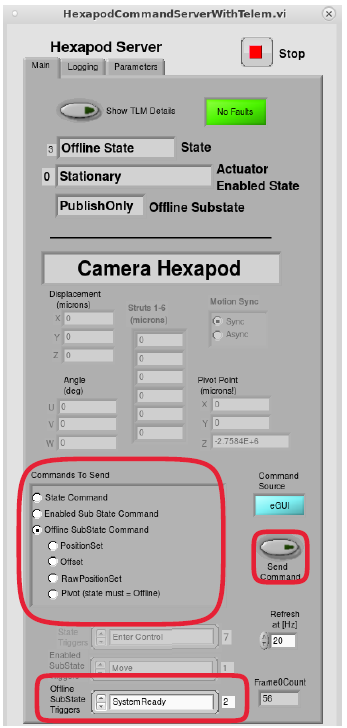
\includegraphics[width=1.79167in]{jira_imgs/1024.png}

\medskip }
\end{minipage}
\\ \cdashline{2-2}


 & Expected Result \\
 & \begin{minipage}[t]{15cm}{\footnotesize
 The system transitions from the OfflineState/PublishOnly substate to the
OfflineState/AvailableState substate and the Command Source says
eGUI.\\[2\baselineskip]

\medskip }
\end{minipage} \\ \cdashline{2-2}

 & Actual Result \\
 & \begin{minipage}[t]{15cm}{\footnotesize

\medskip }
\end{minipage} \\ \cdashline{2-2}

 & Status: \textbf{ Not Executed } \\ \hline

4 & Description \\
 & \begin{minipage}[t]{15cm}
{\footnotesize
 \textbf{OFFLINESTATE -\textgreater{} STANDBYSTATE}\\
Click on the State Command field in the Commands to Send section.\\
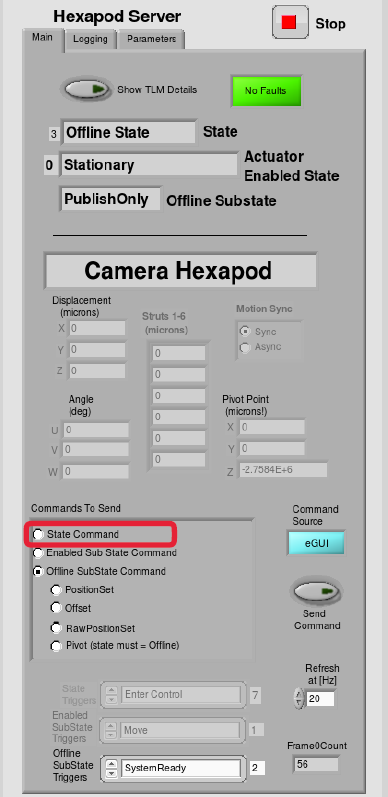
\includegraphics[width=1.79167in]{jira_imgs/1028.png}

\medskip }
\end{minipage}
\\ \cdashline{2-2}


 & Expected Result \\
 & \begin{minipage}[t]{15cm}{\footnotesize
 The State Triggers dialogue box shown below becomes visible.\\
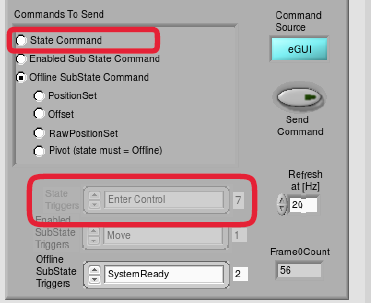
\includegraphics[width=1.79167in]{jira_imgs/1029.png}

\medskip }
\end{minipage} \\ \cdashline{2-2}

 & Actual Result \\
 & \begin{minipage}[t]{15cm}{\footnotesize

\medskip }
\end{minipage} \\ \cdashline{2-2}

 & Status: \textbf{ Not Executed } \\ \hline

5 & Description \\
 & \begin{minipage}[t]{15cm}
{\footnotesize
 Scroll through the available trigger options to select ``Enter Control''
and click the Send Command button.

\medskip }
\end{minipage}
\\ \cdashline{2-2}


 & Expected Result \\
 & \begin{minipage}[t]{15cm}{\footnotesize
 The system transitions to the Standby state and the primary state
display box at the top of the Main says Standby State.

\medskip }
\end{minipage} \\ \cdashline{2-2}

 & Actual Result \\
 & \begin{minipage}[t]{15cm}{\footnotesize

\medskip }
\end{minipage} \\ \cdashline{2-2}

 & Status: \textbf{ Not Executed } \\ \hline

6 & Description \\
 & \begin{minipage}[t]{15cm}
{\footnotesize
 \textbf{STANDBYSTATE -\textgreater{} DISABLEDSTATE}\\
From the StandbyState, send a Start State command.

\medskip }
\end{minipage}
\\ \cdashline{2-2}


 & Expected Result \\
 & \begin{minipage}[t]{15cm}{\footnotesize
 The system transitions into DisabledState and the current configuration
parameters are maintained from the default parameters or from the
previous DDS start command.~

\medskip }
\end{minipage} \\ \cdashline{2-2}

 & Actual Result \\
 & \begin{minipage}[t]{15cm}{\footnotesize

\medskip }
\end{minipage} \\ \cdashline{2-2}

 & Status: \textbf{ Not Executed } \\ \hline

7 & Description \\
 & \begin{minipage}[t]{15cm}
{\footnotesize
 \textbf{DISABLEDSTATE -\textgreater{} ENABLEDSTATE}\\
From the DisabledState, send an Enable State Command.~

\medskip }
\end{minipage}
\\ \cdashline{2-2}


 & Expected Result \\
 & \begin{minipage}[t]{15cm}{\footnotesize
 The system transitions into the EnabledState/Stationary substate, the
motor drives are enabled and and motion can be commanded.~

\medskip }
\end{minipage} \\ \cdashline{2-2}

 & Actual Result \\
 & \begin{minipage}[t]{15cm}{\footnotesize

\medskip }
\end{minipage} \\ \cdashline{2-2}

 & Status: \textbf{ Not Executed } \\ \hline

8 & Description \\
 & \begin{minipage}[t]{15cm}
{\footnotesize
 \textless{}conditional state\textgreater{}\\
\textbf{FAULTSTATE}\\
If a Fault occurs in any of the other states, the system will
automatically transition to the Fault State. While in the Fault state,
send a clearError.\\
Note: If the fault that occurs goes through the interlock system, reset
the safety relay switch and send a clearError command.

\medskip }
\end{minipage}
\\ \cdashline{2-2}


 & Expected Result \\
 & \begin{minipage}[t]{15cm}{\footnotesize
 The system transitions back to the OfflineState/PublishOnly substate.
(Go back to Step 3)

\medskip }
\end{minipage} \\ \cdashline{2-2}

 & Actual Result \\
 & \begin{minipage}[t]{15cm}{\footnotesize

\medskip }
\end{minipage} \\ \cdashline{2-2}

 & Status: \textbf{ Not Executed } \\ \hline

9 & Description \\
 & \begin{minipage}[t]{15cm}
{\footnotesize
 \textbf{Section 3.1.1 of the attached Software Acceptance Test
Procedure\\
Test Sequence \#1 - Synchronous PositionSet and Move
Commands}\\[2\baselineskip]With the synchronous button enabled and in
enabled/stationary state, send a positionSet command of (0um, 0um,
200um, 0 deg, 0 deg, 0 deg) using the EUI.

\medskip }
\end{minipage}
\\ \cdashline{2-2}


 & Expected Result \\
 & \begin{minipage}[t]{15cm}{\footnotesize
 The hexapod doesn't move.

\medskip }
\end{minipage} \\ \cdashline{2-2}

 & Actual Result \\
 & \begin{minipage}[t]{15cm}{\footnotesize

\medskip }
\end{minipage} \\ \cdashline{2-2}

 & Status: \textbf{ Not Executed } \\ \hline

10 & Description \\
 & \begin{minipage}[t]{15cm}
{\footnotesize
 With the synchronous button enabled and in enabled/stationary state,
send a positionSet command of (2000um, -3500um, 200um, .01 deg, -.05deg,
.002deg) using the EUI.

\medskip }
\end{minipage}
\\ \cdashline{2-2}


 & Expected Result \\
 & \begin{minipage}[t]{15cm}{\footnotesize
 The hexapod doesn't move.

\medskip }
\end{minipage} \\ \cdashline{2-2}

 & Actual Result \\
 & \begin{minipage}[t]{15cm}{\footnotesize

\medskip }
\end{minipage} \\ \cdashline{2-2}

 & Status: \textbf{ Not Executed } \\ \hline

11 & Description \\
 & \begin{minipage}[t]{15cm}
{\footnotesize
 Send a move command using the EUI.

\medskip }
\end{minipage}
\\ \cdashline{2-2}


 & Expected Result \\
 & \begin{minipage}[t]{15cm}{\footnotesize
 The hexapod moves to the last commanded position of (2000um, -3500um,
200um, .01 deg, -.05deg, .002deg) and the actuators complete the move at
nearly the same time as seen on the motion complete lights on the
telemetry screen.

\medskip }
\end{minipage} \\ \cdashline{2-2}

 & Actual Result \\
 & \begin{minipage}[t]{15cm}{\footnotesize

\medskip }
\end{minipage} \\ \cdashline{2-2}

 & Status: \textbf{ Not Executed } \\ \hline

12 & Description \\
 & \begin{minipage}[t]{15cm}
{\footnotesize
 \textbf{Section 3.1.1 of the attached Software Acceptance Test
Procedure\\
Test Sequence \#2 - Pivot, PositionSet and Move
Commands}\\[2\baselineskip]In enabled/stationary state and at the last
commanded position of (2000um, -3500um, 200um, .01 deg, -.05deg,
.002deg), change the pivot point from the default location to (0,0,0)
using the EUI.

\medskip }
\end{minipage}
\\ \cdashline{2-2}


 & Expected Result \\
 & \begin{minipage}[t]{15cm}{\footnotesize
 The actuator positions do not change, but the hexapod position is
(-407um, -3982um, 199um, 0.01deg, -0.05deg, 0.002deg)

\medskip }
\end{minipage} \\ \cdashline{2-2}

 & Actual Result \\
 & \begin{minipage}[t]{15cm}{\footnotesize

\medskip }
\end{minipage} \\ \cdashline{2-2}

 & Status: \textbf{ Not Executed } \\ \hline

13 & Description \\
 & \begin{minipage}[t]{15cm}
{\footnotesize
 In the enabled/stationary state, send a positionSet command of (2000um,
-3500um, 200um, .01 deg, -.05deg, .002deg) using the EUI.

\medskip }
\end{minipage}
\\ \cdashline{2-2}


 & Expected Result \\
 & \begin{minipage}[t]{15cm}{\footnotesize
 The hexapod doesn't move.

\medskip }
\end{minipage} \\ \cdashline{2-2}

 & Actual Result \\
 & \begin{minipage}[t]{15cm}{\footnotesize

\medskip }
\end{minipage} \\ \cdashline{2-2}

 & Status: \textbf{ Not Executed } \\ \hline

14 & Description \\
 & \begin{minipage}[t]{15cm}
{\footnotesize
 Send a move command using the EUI.

\medskip }
\end{minipage}
\\ \cdashline{2-2}


 & Expected Result \\
 & \begin{minipage}[t]{15cm}{\footnotesize
 The hexapod moves to the commanded position of (2000um, -3500um, 200um,
.01 deg, -.05deg, .002deg) and the actuators change position to account
for the new pivot point.

\medskip }
\end{minipage} \\ \cdashline{2-2}

 & Actual Result \\
 & \begin{minipage}[t]{15cm}{\footnotesize

\medskip }
\end{minipage} \\ \cdashline{2-2}

 & Status: \textbf{ Not Executed } \\ \hline

15 & Description \\
 & \begin{minipage}[t]{15cm}
{\footnotesize
 \textbf{Section 3.1.1 of the attached Software Acceptance Test
Procedure\\
Test Sequence \#4 - Synchronous Offset and Move
Commands}\\[2\baselineskip]With the synchronous button enabled and in
enabled/stationary state, send a positionSet command of (500um, 800um,
200um, 0 deg, 0 deg, 0 deg).

\medskip }
\end{minipage}
\\ \cdashline{2-2}


 & Expected Result \\
 & \begin{minipage}[t]{15cm}{\footnotesize
 The hexapod doesn't move.

\medskip }
\end{minipage} \\ \cdashline{2-2}

 & Actual Result \\
 & \begin{minipage}[t]{15cm}{\footnotesize

\medskip }
\end{minipage} \\ \cdashline{2-2}

 & Status: \textbf{ Not Executed } \\ \hline

16 & Description \\
 & \begin{minipage}[t]{15cm}
{\footnotesize
 With the synchronous button enabled and in enabled/stationary state,
send an offset command of (0um, 0um, 2000um, 0 deg, 0 deg, 0 deg).~

\medskip }
\end{minipage}
\\ \cdashline{2-2}


 & Expected Result \\
 & \begin{minipage}[t]{15cm}{\footnotesize
 The hexapod doesn't move.

\medskip }
\end{minipage} \\ \cdashline{2-2}

 & Actual Result \\
 & \begin{minipage}[t]{15cm}{\footnotesize

\medskip }
\end{minipage} \\ \cdashline{2-2}

 & Status: \textbf{ Not Executed } \\ \hline

17 & Description \\
 & \begin{minipage}[t]{15cm}
{\footnotesize
 Send a move command.

\medskip }
\end{minipage}
\\ \cdashline{2-2}


 & Expected Result \\
 & \begin{minipage}[t]{15cm}{\footnotesize
 The hexapod moves only 2000um in Z from the previous position and the
actuators complete the move at nearly the same time as seen on the
motion complete lights on the telemetry screen.

\medskip }
\end{minipage} \\ \cdashline{2-2}

 & Actual Result \\
 & \begin{minipage}[t]{15cm}{\footnotesize

\medskip }
\end{minipage} \\ \cdashline{2-2}

 & Status: \textbf{ Not Executed } \\ \hline

18 & Description \\
 & \begin{minipage}[t]{15cm}
{\footnotesize
 \textbf{Instead of Asynchronous Test}\\
{With the synchronous button enabled and in enabled/stationary
state,}{\textbf{~}}{s}end a position set command of (0um, 0um, 0um,
0.1deg, 0deg, 0deg)

\medskip }
\end{minipage}
\\ \cdashline{2-2}


 & Expected Result \\
 & \begin{minipage}[t]{15cm}{\footnotesize
 The hexapod doesn't move.

\medskip }
\end{minipage} \\ \cdashline{2-2}

 & Actual Result \\
 & \begin{minipage}[t]{15cm}{\footnotesize

\medskip }
\end{minipage} \\ \cdashline{2-2}

 & Status: \textbf{ Not Executed } \\ \hline

19 & Description \\
 & \begin{minipage}[t]{15cm}
{\footnotesize
 Send a move command.

\medskip }
\end{minipage}
\\ \cdashline{2-2}


 & Expected Result \\
 & \begin{minipage}[t]{15cm}{\footnotesize
 The hexapod moves to the commanded position of (0um, 0um, 0um, 0.1deg,
0deg, 0deg)

\medskip }
\end{minipage} \\ \cdashline{2-2}

 & Actual Result \\
 & \begin{minipage}[t]{15cm}{\footnotesize

\medskip }
\end{minipage} \\ \cdashline{2-2}

 & Status: \textbf{ Not Executed } \\ \hline

20 & Description \\
 & \begin{minipage}[t]{15cm}
{\footnotesize
 With the synchronous button enabled and in enabled/stationary
state,\textbf{~}send a position set command of (0um, 0um, 0um, 0deg,
0.1deg, 0deg)

\medskip }
\end{minipage}
\\ \cdashline{2-2}


 & Expected Result \\
 & \begin{minipage}[t]{15cm}{\footnotesize
 The hexapod doesn't move.

\medskip }
\end{minipage} \\ \cdashline{2-2}

 & Actual Result \\
 & \begin{minipage}[t]{15cm}{\footnotesize

\medskip }
\end{minipage} \\ \cdashline{2-2}

 & Status: \textbf{ Not Executed } \\ \hline

21 & Description \\
 & \begin{minipage}[t]{15cm}
{\footnotesize
 Send a move command.

\medskip }
\end{minipage}
\\ \cdashline{2-2}


 & Expected Result \\
 & \begin{minipage}[t]{15cm}{\footnotesize
 The hexapod moves to the commanded position of (0um, 0um, 0um, 0deg,
0.1deg, 0deg)

\medskip }
\end{minipage} \\ \cdashline{2-2}

 & Actual Result \\
 & \begin{minipage}[t]{15cm}{\footnotesize

\medskip }
\end{minipage} \\ \cdashline{2-2}

 & Status: \textbf{ Not Executed } \\ \hline

22 & Description \\
 & \begin{minipage}[t]{15cm}
{\footnotesize
 With the synchronous button enabled and in enabled/stationary
state,\textbf{~}send a position set command of (0um, 0um, 0um, 0.1deg,
0.1deg, 0deg)

\medskip }
\end{minipage}
\\ \cdashline{2-2}


 & Expected Result \\
 & \begin{minipage}[t]{15cm}{\footnotesize
 The hexapod doesn't move.

\medskip }
\end{minipage} \\ \cdashline{2-2}

 & Actual Result \\
 & \begin{minipage}[t]{15cm}{\footnotesize

\medskip }
\end{minipage} \\ \cdashline{2-2}

 & Status: \textbf{ Not Executed } \\ \hline

23 & Description \\
 & \begin{minipage}[t]{15cm}
{\footnotesize
 Send a move command.

\medskip }
\end{minipage}
\\ \cdashline{2-2}


 & Expected Result \\
 & \begin{minipage}[t]{15cm}{\footnotesize
 The hexapod moves to the commanded position of (0um, 0um, 0um, 0.1deg,
0.1deg, 0deg)

\medskip }
\end{minipage} \\ \cdashline{2-2}

 & Actual Result \\
 & \begin{minipage}[t]{15cm}{\footnotesize

\medskip }
\end{minipage} \\ \cdashline{2-2}

 & Status: \textbf{ Not Executed } \\ \hline

24 & Description \\
 & \begin{minipage}[t]{15cm}
{\footnotesize
 \textbf{Section 3.1.1 of the attached Software Acceptance Test
Procedure\\
Test Sequence \#5 - Stop Commands}\\[2\baselineskip]In
enabled/stationary state, send a position set command of (0um, 0um,
5000um, 0 deg, 0 deg, 0 deg).

\medskip }
\end{minipage}
\\ \cdashline{2-2}


 & Expected Result \\
 & \begin{minipage}[t]{15cm}{\footnotesize
 The hexapod doesn't move.

\medskip }
\end{minipage} \\ \cdashline{2-2}

 & Actual Result \\
 & \begin{minipage}[t]{15cm}{\footnotesize

\medskip }
\end{minipage} \\ \cdashline{2-2}

 & Status: \textbf{ Not Executed } \\ \hline

25 & Description \\
 & \begin{minipage}[t]{15cm}
{\footnotesize
 Send a move command.

\medskip }
\end{minipage}
\\ \cdashline{2-2}


 & Expected Result \\
 & \begin{minipage}[t]{15cm}{\footnotesize
 The hexapod starts to move to the commanded position.

\medskip }
\end{minipage} \\ \cdashline{2-2}

 & Actual Result \\
 & \begin{minipage}[t]{15cm}{\footnotesize

\medskip }
\end{minipage} \\ \cdashline{2-2}

 & Status: \textbf{ Not Executed } \\ \hline

26 & Description \\
 & \begin{minipage}[t]{15cm}
{\footnotesize
 While the hexapod is moving, send a stop command.~

\medskip }
\end{minipage}
\\ \cdashline{2-2}


 & Expected Result \\
 & \begin{minipage}[t]{15cm}{\footnotesize
 The hexapod quickly comes to a stop prior to reaching the commanded
position.

\medskip }
\end{minipage} \\ \cdashline{2-2}

 & Actual Result \\
 & \begin{minipage}[t]{15cm}{\footnotesize

\medskip }
\end{minipage} \\ \cdashline{2-2}

 & Status: \textbf{ Not Executed } \\ \hline

27 & Description \\
 & \begin{minipage}[t]{15cm}
{\footnotesize
 \textbf{Section 3.3.1 EUI Tests of the attached Software Acceptance Test
Procedure}\\
At startup, confirm that the system starts in the Offline/PublishOnly
state.

\medskip }
\end{minipage}
\\ \cdashline{2-2}


 & Expected Result \\
 & \begin{minipage}[t]{15cm}{\footnotesize
 The rotator starts in the Offline/PublishOnly state.

\medskip }
\end{minipage} \\ \cdashline{2-2}

 & Actual Result \\
 & \begin{minipage}[t]{15cm}{\footnotesize

\medskip }
\end{minipage} \\ \cdashline{2-2}

 & Status: \textbf{ Not Executed } \\ \hline

28 & Description \\
 & \begin{minipage}[t]{15cm}
{\footnotesize
 Send an offline substate trigger of systemReady.

\medskip }
\end{minipage}
\\ \cdashline{2-2}


 & Expected Result \\
 & \begin{minipage}[t]{15cm}{\footnotesize
 The system transitions into the Offline/Available substate.

\medskip }
\end{minipage} \\ \cdashline{2-2}

 & Actual Result \\
 & \begin{minipage}[t]{15cm}{\footnotesize

\medskip }
\end{minipage} \\ \cdashline{2-2}

 & Status: \textbf{ Not Executed } \\ \hline

29 & Description \\
 & \begin{minipage}[t]{15cm}
{\footnotesize
 Send an EnterControl trigger.

\medskip }
\end{minipage}
\\ \cdashline{2-2}


 & Expected Result \\
 & \begin{minipage}[t]{15cm}{\footnotesize
 The system transitions from Offline/Available to Standby state.

\medskip }
\end{minipage} \\ \cdashline{2-2}

 & Actual Result \\
 & \begin{minipage}[t]{15cm}{\footnotesize

\medskip }
\end{minipage} \\ \cdashline{2-2}

 & Status: \textbf{ Not Executed } \\ \hline

30 & Description \\
 & \begin{minipage}[t]{15cm}
{\footnotesize
 Send a Start trigger.

\medskip }
\end{minipage}
\\ \cdashline{2-2}


 & Expected Result \\
 & \begin{minipage}[t]{15cm}{\footnotesize
 The system transitions from Standby to Disabled state.

\medskip }
\end{minipage} \\ \cdashline{2-2}

 & Actual Result \\
 & \begin{minipage}[t]{15cm}{\footnotesize

\medskip }
\end{minipage} \\ \cdashline{2-2}

 & Status: \textbf{ Not Executed } \\ \hline

31 & Description \\
 & \begin{minipage}[t]{15cm}
{\footnotesize
 Send an Enable trigger.

\medskip }
\end{minipage}
\\ \cdashline{2-2}


 & Expected Result \\
 & \begin{minipage}[t]{15cm}{\footnotesize
 The system transitions from Disabled to Enabled state.

\medskip }
\end{minipage} \\ \cdashline{2-2}

 & Actual Result \\
 & \begin{minipage}[t]{15cm}{\footnotesize

\medskip }
\end{minipage} \\ \cdashline{2-2}

 & Status: \textbf{ Not Executed } \\ \hline

32 & Description \\
 & \begin{minipage}[t]{15cm}
{\footnotesize
 Send a Disable trigger.

\medskip }
\end{minipage}
\\ \cdashline{2-2}


 & Expected Result \\
 & \begin{minipage}[t]{15cm}{\footnotesize
 The system transitions from Enabled to Disabled state.

\medskip }
\end{minipage} \\ \cdashline{2-2}

 & Actual Result \\
 & \begin{minipage}[t]{15cm}{\footnotesize

\medskip }
\end{minipage} \\ \cdashline{2-2}

 & Status: \textbf{ Not Executed } \\ \hline

33 & Description \\
 & \begin{minipage}[t]{15cm}
{\footnotesize
 Send a Standby trigger.

\medskip }
\end{minipage}
\\ \cdashline{2-2}


 & Expected Result \\
 & \begin{minipage}[t]{15cm}{\footnotesize
 The system transitions from Disabled state to Standby state.

\medskip }
\end{minipage} \\ \cdashline{2-2}

 & Actual Result \\
 & \begin{minipage}[t]{15cm}{\footnotesize

\medskip }
\end{minipage} \\ \cdashline{2-2}

 & Status: \textbf{ Not Executed } \\ \hline

34 & Description \\
 & \begin{minipage}[t]{15cm}
{\footnotesize
 Send a exitControl trigger.

\medskip }
\end{minipage}
\\ \cdashline{2-2}


 & Expected Result \\
 & \begin{minipage}[t]{15cm}{\footnotesize
 The system transitions from Standby state to Offline state.

\medskip }
\end{minipage} \\ \cdashline{2-2}

 & Actual Result \\
 & \begin{minipage}[t]{15cm}{\footnotesize

\medskip }
\end{minipage} \\ \cdashline{2-2}

 & Status: \textbf{ Not Executed } \\ \hline

35 & Description \\
 & \begin{minipage}[t]{15cm}
{\footnotesize
 Return to the Enabled state and trip the safety interlock switch.

\medskip }
\end{minipage}
\\ \cdashline{2-2}


 & Expected Result \\
 & \begin{minipage}[t]{15cm}{\footnotesize
 The system transitions to Fault state.

\medskip }
\end{minipage} \\ \cdashline{2-2}

 & Actual Result \\
 & \begin{minipage}[t]{15cm}{\footnotesize

\medskip }
\end{minipage} \\ \cdashline{2-2}

 & Status: \textbf{ Not Executed } \\ \hline

36 & Description \\
 & \begin{minipage}[t]{15cm}
{\footnotesize
 Reset the safety interlock and send a ClearError trigger.

\medskip }
\end{minipage}
\\ \cdashline{2-2}


 & Expected Result \\
 & \begin{minipage}[t]{15cm}{\footnotesize
 The system transitions from Fault state to Offline state

\medskip }
\end{minipage} \\ \cdashline{2-2}

 & Actual Result \\
 & \begin{minipage}[t]{15cm}{\footnotesize

\medskip }
\end{minipage} \\ \cdashline{2-2}

 & Status: \textbf{ Not Executed } \\ \hline

37 & Description \\
 & \begin{minipage}[t]{15cm}
{\footnotesize
 \textbf{Section 4.1 Hexapod Events of the attached Software Acceptance
Test Procedure}\\[2\baselineskip]In the Enabled/Stationary state, unplug
a motor encoder cable for one of the actuators.

\medskip }
\end{minipage}
\\ \cdashline{2-2}

 & Test Data \\
 & \begin{minipage}[t]{15cm}{\footnotesize
 \textbf{Deviation:~}Perform the following set of steps using the EUI
instead of the DDS and verify the events are displayed on the EUI.

\medskip }
\end{minipage} \\ \cdashline{2-2}

 & Expected Result \\
 & \begin{minipage}[t]{15cm}{\footnotesize
 A Drive Fault error event is created and the system transitions to Fault
state.

\medskip }
\end{minipage} \\ \cdashline{2-2}

 & Actual Result \\
 & \begin{minipage}[t]{15cm}{\footnotesize

\medskip }
\end{minipage} \\ \cdashline{2-2}

 & Status: \textbf{ Not Executed } \\ \hline

38 & Description \\
 & \begin{minipage}[t]{15cm}
{\footnotesize
 In the Enabled/Stationary state, unplug a linear encoder cable for one
of the actuators.~

\medskip }
\end{minipage}
\\ \cdashline{2-2}


 & Expected Result \\
 & \begin{minipage}[t]{15cm}{\footnotesize
 A Drive Fault error event is created and the system transitions to Fault
state.

\medskip }
\end{minipage} \\ \cdashline{2-2}

 & Actual Result \\
 & \begin{minipage}[t]{15cm}{\footnotesize

\medskip }
\end{minipage} \\ \cdashline{2-2}

 & Status: \textbf{ Not Executed } \\ \hline

39 & Description \\
 & \begin{minipage}[t]{15cm}
{\footnotesize
 Unplug a motor power cable from one of the actuators and command a
PositionSet/Move.~

\medskip }
\end{minipage}
\\ \cdashline{2-2}


 & Expected Result \\
 & \begin{minipage}[t]{15cm}{\footnotesize
 A Following Error event is created and the system transitions to Fault
state.

\medskip }
\end{minipage} \\ \cdashline{2-2}

 & Actual Result \\
 & \begin{minipage}[t]{15cm}{\footnotesize

\medskip }
\end{minipage} \\ \cdashline{2-2}

 & Status: \textbf{ Not Executed } \\ \hline

40 & Description \\
 & \begin{minipage}[t]{15cm}
{\footnotesize
 Activate an extension limit switch on one of the actuators by removing
the limit switch cover and manually tripping.~

\medskip }
\end{minipage}
\\ \cdashline{2-2}


 & Expected Result \\
 & \begin{minipage}[t]{15cm}{\footnotesize
 An Extended Limit Switch error event is created and the system
transitions into Fault state.

\medskip }
\end{minipage} \\ \cdashline{2-2}

 & Actual Result \\
 & \begin{minipage}[t]{15cm}{\footnotesize

\medskip }
\end{minipage} \\ \cdashline{2-2}

 & Status: \textbf{ Not Executed } \\ \hline

41 & Description \\
 & \begin{minipage}[t]{15cm}
{\footnotesize
 Activate a retraction limit switch on one of the actuators by removing
the limit switch cover and manually tripping.

\medskip }
\end{minipage}
\\ \cdashline{2-2}


 & Expected Result \\
 & \begin{minipage}[t]{15cm}{\footnotesize
 A Retracted Limit Switch error event is created and the system
transitions into Fault state.

\medskip }
\end{minipage} \\ \cdashline{2-2}

 & Actual Result \\
 & \begin{minipage}[t]{15cm}{\footnotesize

\medskip }
\end{minipage} \\ \cdashline{2-2}

 & Status: \textbf{ Not Executed } \\ \hline

42 & Description \\
 & \begin{minipage}[t]{15cm}
{\footnotesize
 Unplug the Ethercat cable between the control PC and the first Copley
XE2 drive.

\medskip }
\end{minipage}
\\ \cdashline{2-2}


 & Expected Result \\
 & \begin{minipage}[t]{15cm}{\footnotesize
 An Ethercat Lost event is created and the system transitions to Fault
state.

\medskip }
\end{minipage} \\ \cdashline{2-2}

 & Actual Result \\
 & \begin{minipage}[t]{15cm}{\footnotesize

\medskip }
\end{minipage} \\ \cdashline{2-2}

 & Status: \textbf{ Not Executed } \\ \hline

\end{longtable}

\paragraph{Test Case LVV-T1800 - M2 Hexapod Hardware Functional Re-verification }\mbox{}\\

Open  \href{https://jira.lsstcorp.org/secure/Tests.jspa#/testCase/LVV-T1800}{\textit{ LVV-T1800 } }
test case in Jira.

The objective of this test case is to re-verify the functional
requirements of the M2 hexapod's hardware, after shipment from the
vendor's facility to the Summit, as defined in \citeds{LTS-206}. This test case
will only exercise the functionality that was executed previously and
meets the following criteria:

\begin{itemize}
\tightlist
\item
  Only requires the M2 hexapod to be operable
\item
  Only requires the EUI software and hardware via local control
\item
  Only requires a laser tracker
\item
  Does require the M2 hexapod temperature sensors be operating
\item
  Does \textbf{NOT} require the M2 hexapod to be loaded with an M2
  simulated mass or actual M2
\item
  Does \textbf{NOT} require the M2 hexapod to be rotated to various
  elevation angles
\item
  Does \textbf{NOT~}require the M2 hexapod be in a climate controlled
  environment
\end{itemize}

\textbf{ Preconditions}:\\
Prior to the execution of this test case to re-verify the M2 Hexapod
hardware functional requirements, the following Summit tasks must be
completed:

\begin{itemize}
\tightlist
\item
  The measurement equipment has been set-up for testing

  \begin{itemize}
  \tightlist
  \item
    \url{https://jira.lsstcorp.org/browse/SUMMIT-1943}
  \end{itemize}
\item
  The laser tracker has been set up for measurements

  \begin{itemize}
  \tightlist
  \item
    \url{https://jira.lsstcorp.org/browse/SUMMIT-3951}
  \end{itemize}
\end{itemize}

Execution status: {\bf Not Executed }

Final comment:\\


Detailed steps results:

\begin{longtable}{p{1cm}p{15cm}}
\hline
{Step} & Step Details\\ \hline
1 & Description \\
 & \begin{minipage}[t]{15cm}
{\footnotesize
 \textbf{STARTING THE EUI}\\[2\baselineskip]Double click the Hexapod GUI
Viewer desktop icon on the computer.

\begin{itemize}
\tightlist
\item
  This can be done on the Dell Management PC or another computer on the
  same network
\end{itemize}

\medskip }
\end{minipage}
\\ \cdashline{2-2}


 & Expected Result \\
 & \begin{minipage}[t]{15cm}{\footnotesize
 A prompt to enter the password is shown.

\medskip }
\end{minipage} \\ \cdashline{2-2}

 & Actual Result \\
 & \begin{minipage}[t]{15cm}{\footnotesize

\medskip }
\end{minipage} \\ \cdashline{2-2}

 & Status: \textbf{ Not Executed } \\ \hline

2 & Description \\
 & \begin{minipage}[t]{15cm}
{\footnotesize
 Enter the password ``lsst-vnc''

\begin{itemize}
\tightlist
\item
  If the EUI isn't automatically up and running when the VNC opens,
  double click on the Hexapod-eGUI icon on the VNC viewer
\end{itemize}

\medskip }
\end{minipage}
\\ \cdashline{2-2}


 & Expected Result \\
 & \begin{minipage}[t]{15cm}{\footnotesize
 The EUI is in the Offline State/PublishOnly substate and is able to
publish through SAL but cannot receive commands.

\medskip }
\end{minipage} \\ \cdashline{2-2}

 & Actual Result \\
 & \begin{minipage}[t]{15cm}{\footnotesize

\medskip }
\end{minipage} \\ \cdashline{2-2}

 & Status: \textbf{ Not Executed } \\ \hline

3 & Description \\
 & \begin{minipage}[t]{15cm}
{\footnotesize
 \textbf{OFFLINESTATE/AVAILABLESTATE}\\
On the Main tab, select the ``Offline SubState Cmd'' field in the
Commands to Send section, set the Offline SubState Triggers to ``System
Ready'' and click on the Send Command button.\\
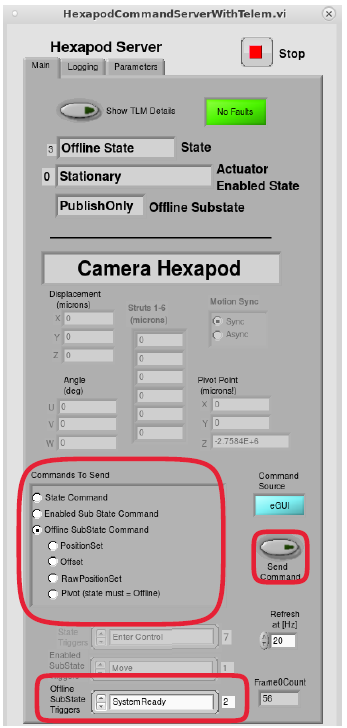
\includegraphics[width=1.79167in]{jira_imgs/1024.png}

\medskip }
\end{minipage}
\\ \cdashline{2-2}


 & Expected Result \\
 & \begin{minipage}[t]{15cm}{\footnotesize
 The system transitions from the OfflineState/PublishOnly substate to the
OfflineState/AvailableState substate and the Command Source says
eGUI.\\[2\baselineskip]

\medskip }
\end{minipage} \\ \cdashline{2-2}

 & Actual Result \\
 & \begin{minipage}[t]{15cm}{\footnotesize

\medskip }
\end{minipage} \\ \cdashline{2-2}

 & Status: \textbf{ Not Executed } \\ \hline

4 & Description \\
 & \begin{minipage}[t]{15cm}
{\footnotesize
 \textbf{OFFLINESTATE -\textgreater{} STANDBYSTATE}\\
Click on the State Command field in the Commands to Send section.\\
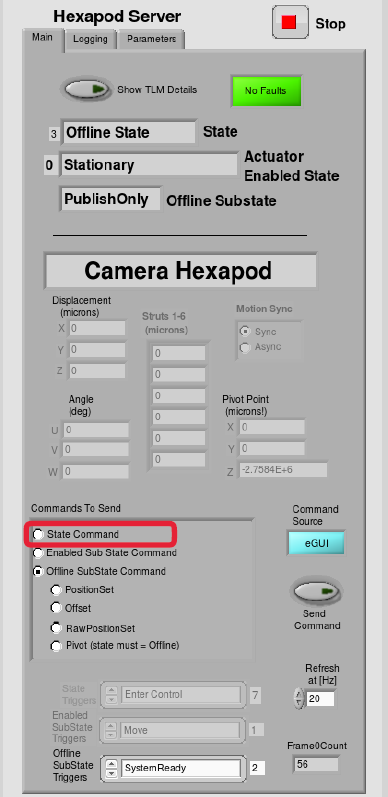
\includegraphics[width=1.79167in]{jira_imgs/1028.png}

\medskip }
\end{minipage}
\\ \cdashline{2-2}


 & Expected Result \\
 & \begin{minipage}[t]{15cm}{\footnotesize
 The State Triggers dialogue box shown below becomes visible.\\
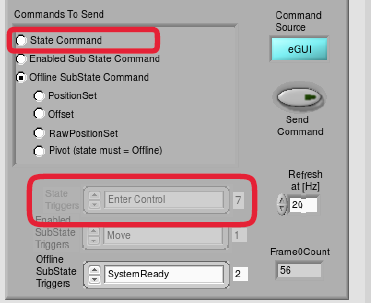
\includegraphics[width=1.79167in]{jira_imgs/1029.png}

\medskip }
\end{minipage} \\ \cdashline{2-2}

 & Actual Result \\
 & \begin{minipage}[t]{15cm}{\footnotesize

\medskip }
\end{minipage} \\ \cdashline{2-2}

 & Status: \textbf{ Not Executed } \\ \hline

5 & Description \\
 & \begin{minipage}[t]{15cm}
{\footnotesize
 Scroll through the available trigger options to select ``Enter Control''
and click the Send Command button.

\medskip }
\end{minipage}
\\ \cdashline{2-2}


 & Expected Result \\
 & \begin{minipage}[t]{15cm}{\footnotesize
 The system transitions to the Standby state and the primary state
display box at the top of the Main says Standby State.

\medskip }
\end{minipage} \\ \cdashline{2-2}

 & Actual Result \\
 & \begin{minipage}[t]{15cm}{\footnotesize

\medskip }
\end{minipage} \\ \cdashline{2-2}

 & Status: \textbf{ Not Executed } \\ \hline

6 & Description \\
 & \begin{minipage}[t]{15cm}
{\footnotesize
 \textbf{STANDBYSTATE -\textgreater{} DISABLEDSTATE}\\
From the StandbyState, send a Start State command.

\medskip }
\end{minipage}
\\ \cdashline{2-2}


 & Expected Result \\
 & \begin{minipage}[t]{15cm}{\footnotesize
 The system transitions into DisabledState and the current configuration
parameters are maintained from the default parameters or from the
previous DDS start command.~

\medskip }
\end{minipage} \\ \cdashline{2-2}

 & Actual Result \\
 & \begin{minipage}[t]{15cm}{\footnotesize

\medskip }
\end{minipage} \\ \cdashline{2-2}

 & Status: \textbf{ Not Executed } \\ \hline

7 & Description \\
 & \begin{minipage}[t]{15cm}
{\footnotesize
 \textbf{DISABLEDSTATE -\textgreater{} ENABLEDSTATE}\\
From the DisabledState, send an Enable State Command.~

\medskip }
\end{minipage}
\\ \cdashline{2-2}


 & Expected Result \\
 & \begin{minipage}[t]{15cm}{\footnotesize
 The system transitions into the EnabledState/Stationary substate, the
motor drives are enabled and and motion can be commanded.~

\medskip }
\end{minipage} \\ \cdashline{2-2}

 & Actual Result \\
 & \begin{minipage}[t]{15cm}{\footnotesize

\medskip }
\end{minipage} \\ \cdashline{2-2}

 & Status: \textbf{ Not Executed } \\ \hline

8 & Description \\
 & \begin{minipage}[t]{15cm}
{\footnotesize
 \textless{}conditional state\textgreater{}\\
\textbf{FAULTSTATE}\\
If a Fault occurs in any of the other states, the system will
automatically transition to the Fault State. While in the Fault state,
send a clearError.\\
Note: If the fault that occurs goes through the interlock system, reset
the safety relay switch and send a clearError command.

\medskip }
\end{minipage}
\\ \cdashline{2-2}


 & Expected Result \\
 & \begin{minipage}[t]{15cm}{\footnotesize
 The system transitions back to the OfflineState/PublishOnly substate.
(Go back to Step 3)

\medskip }
\end{minipage} \\ \cdashline{2-2}

 & Actual Result \\
 & \begin{minipage}[t]{15cm}{\footnotesize

\medskip }
\end{minipage} \\ \cdashline{2-2}

 & Status: \textbf{ Not Executed } \\ \hline

9 & Description \\
 & \begin{minipage}[t]{15cm}
{\footnotesize
 \textbf{Follow \emph{3.5.12 Positioning~}of the LSST Hexapods-Rotator
Acceptance Test Procedure, Sheet 57-58.}

\medskip }
\end{minipage}
\\ \cdashline{2-2}

 & Test Data \\
 & \begin{minipage}[t]{15cm}{\footnotesize
 \textbf{Deviation}: Test at a single elevation angle and with no
performance payload.

\medskip }
\end{minipage} \\ \cdashline{2-2}

 & Expected Result \\
 & \begin{minipage}[t]{15cm}{\footnotesize
 The position of the hexapod is able to reach the commanded positions
within the absolute accuracy specifications of 25um in Z, 125um in XY,
83x10-5deg in RXRY, and 750x10-5deg in RZ.

\medskip }
\end{minipage} \\ \cdashline{2-2}

 & Actual Result \\
 & \begin{minipage}[t]{15cm}{\footnotesize

\medskip }
\end{minipage} \\ \cdashline{2-2}

 & Status: \textbf{ Not Executed } \\ \hline

10 & Description \\
 & \begin{minipage}[t]{15cm}
{\footnotesize
 \textbf{Follow \emph{3.5.13 Centers of Rotation~}of the LSST
Hexapods-Rotator Acceptance Test Procedure, Sheet 58-59.}

\medskip }
\end{minipage}
\\ \cdashline{2-2}

 & Test Data \\
 & \begin{minipage}[t]{15cm}{\footnotesize
 \textbf{Deviation}: Test at a single elevation angle and with no
performance payload.

\medskip }
\end{minipage} \\ \cdashline{2-2}

 & Expected Result \\
 & \begin{minipage}[t]{15cm}{\footnotesize
 The center of rotation is able to be moved.

\medskip }
\end{minipage} \\ \cdashline{2-2}

 & Actual Result \\
 & \begin{minipage}[t]{15cm}{\footnotesize

\medskip }
\end{minipage} \\ \cdashline{2-2}

 & Status: \textbf{ Not Executed } \\ \hline

11 & Description \\
 & \begin{minipage}[t]{15cm}
{\footnotesize
 \textbf{Follow \emph{3.5.15 Radial (X and Y) Translation Range~}of
the}~\textbf{LSST Hexapods-Rotator Acceptance Test Procedure, Sheet 59.}

\medskip }
\end{minipage}
\\ \cdashline{2-2}

 & Test Data \\
 & \begin{minipage}[t]{15cm}{\footnotesize
 \textbf{Deviation}: Test at a single elevation angle and with no
performance payload.

\medskip }
\end{minipage} \\ \cdashline{2-2}

 & Expected Result \\
 & \begin{minipage}[t]{15cm}{\footnotesize
 The hexapod is capable of moving to the positions in the XY plane listed
in the Acceptance Test Procedure.

\medskip }
\end{minipage} \\ \cdashline{2-2}

 & Actual Result \\
 & \begin{minipage}[t]{15cm}{\footnotesize

\medskip }
\end{minipage} \\ \cdashline{2-2}

 & Status: \textbf{ Not Executed } \\ \hline

12 & Description \\
 & \begin{minipage}[t]{15cm}
{\footnotesize
 \textbf{Follow \emph{3.5.17 Axial (Z) Translation Range~}of the}
\textbf{LSST Hexapods-Rotator Acceptance Test Procedure, Sheet 60.}

\medskip }
\end{minipage}
\\ \cdashline{2-2}

 & Test Data \\
 & \begin{minipage}[t]{15cm}{\footnotesize
 \textbf{Deviation}: Test at a single elevation angle and with no
performance payload.

\medskip }
\end{minipage} \\ \cdashline{2-2}

 & Expected Result \\
 & \begin{minipage}[t]{15cm}{\footnotesize
 The hexapod is capable of moving to the positions in the Z plane listed
in the Acceptance Test Procedure.

\medskip }
\end{minipage} \\ \cdashline{2-2}

 & Actual Result \\
 & \begin{minipage}[t]{15cm}{\footnotesize

\medskip }
\end{minipage} \\ \cdashline{2-2}

 & Status: \textbf{ Not Executed } \\ \hline

13 & Description \\
 & \begin{minipage}[t]{15cm}
{\footnotesize
 \textbf{Follow \emph{3.5.19 Rotational Range Around X-Axis (Tip) and
Y-Axis (Tilt)~}of the} \textbf{LSST Hexapods-Rotator Acceptance Test
Procedure, Sheet 61.}

\medskip }
\end{minipage}
\\ \cdashline{2-2}

 & Test Data \\
 & \begin{minipage}[t]{15cm}{\footnotesize
 \textbf{Deviation}: Test at a single elevation angle and with no
performance payload.

\medskip }
\end{minipage} \\ \cdashline{2-2}

 & Expected Result \\
 & \begin{minipage}[t]{15cm}{\footnotesize
 The hexapod is capable of moving to the positions in the RXRY plane
listed in the Acceptance Test Procedure.

\medskip }
\end{minipage} \\ \cdashline{2-2}

 & Actual Result \\
 & \begin{minipage}[t]{15cm}{\footnotesize

\medskip }
\end{minipage} \\ \cdashline{2-2}

 & Status: \textbf{ Not Executed } \\ \hline

14 & Description \\
 & \begin{minipage}[t]{15cm}
{\footnotesize
 \textbf{Follow \emph{3.5.21 Rotation Range Around Z-Axis (Twist)~}of
the} \textbf{LSST Hexapods-Rotator Acceptance Test Procedure, Sheet 62.}

\medskip }
\end{minipage}
\\ \cdashline{2-2}

 & Test Data \\
 & \begin{minipage}[t]{15cm}{\footnotesize
 \textbf{Deviation}: Test at a single elevation angle and with no
performance payload.

\medskip }
\end{minipage} \\ \cdashline{2-2}

 & Expected Result \\
 & \begin{minipage}[t]{15cm}{\footnotesize
 The hexapod is capable of moving to the positions in the RZ-axis listed
in the Acceptance Test Procedure.

\medskip }
\end{minipage} \\ \cdashline{2-2}

 & Actual Result \\
 & \begin{minipage}[t]{15cm}{\footnotesize

\medskip }
\end{minipage} \\ \cdashline{2-2}

 & Status: \textbf{ Not Executed } \\ \hline

15 & Description \\
 & \begin{minipage}[t]{15cm}
{\footnotesize
 \textbf{Follow \emph{3.5.23 Hexapod Repeatability~}of the} \textbf{LSST
Hexapods-Rotator Acceptance Test Procedure, Sheet 63-70.}

\medskip }
\end{minipage}
\\ \cdashline{2-2}

 & Test Data \\
 & \begin{minipage}[t]{15cm}{\footnotesize
 \textbf{Deviation}: Allow a minimum of 30 seconds between moves

\medskip }
\end{minipage} \\ \cdashline{2-2}

 & Expected Result \\
 & \begin{minipage}[t]{15cm}{\footnotesize
 The repeatability of the hexapod is likely better than can be determined
by the test equipment. This test will likely falsely show a deficiency
in the hexapod performance as a result of test equipment accuracy/
repeatability limitation.

\medskip }
\end{minipage} \\ \cdashline{2-2}

 & Actual Result \\
 & \begin{minipage}[t]{15cm}{\footnotesize

\medskip }
\end{minipage} \\ \cdashline{2-2}

 & Status: \textbf{ Not Executed } \\ \hline

16 & Description \\
 & \begin{minipage}[t]{15cm}
{\footnotesize
 \textbf{Follow \emph{3.5.24 Hexapod Absolute Accuracy~}of the}
\textbf{LSST Hexapods-Rotator Acceptance Test Procedure, Sheet 70-74.}

\medskip }
\end{minipage}
\\ \cdashline{2-2}

 & Test Data \\
 & \begin{minipage}[t]{15cm}{\footnotesize
 \textbf{Deviation}: Test at a single elevation angle and with no
performance payload.

\medskip }
\end{minipage} \\ \cdashline{2-2}

 & Expected Result \\
 & \begin{minipage}[t]{15cm}{\footnotesize
 The accuracy of the hexapod is at least the following:\\[2\baselineskip]

\begin{tabular}[]{@{}ll@{}}
\toprule
Axis & Required Accuracy (um, deg)\tabularnewline
\midrule
%\endhead
X & 125\tabularnewline
Y & 125\tabularnewline
Z & 25\tabularnewline
RX & 0.00083\tabularnewline
RY & 0.00083\tabularnewline
RZ & 0.0075\tabularnewline
\bottomrule
\end{tabular}\\[\baselineskip]

\textbf{NOTE:~}The accuracy of the hexapod may be better than can be
determined by the test equipment. This may falsely show a deficiency in
the hexapod performance as a result of test equipment accuracy/
repeatability limitation.~

\medskip }
\end{minipage} \\ \cdashline{2-2}

 & Actual Result \\
 & \begin{minipage}[t]{15cm}{\footnotesize

\medskip }
\end{minipage} \\ \cdashline{2-2}

 & Status: \textbf{ Not Executed } \\ \hline

17 & Description \\
 & \begin{minipage}[t]{15cm}
{\footnotesize
 \textbf{Follow \emph{3.5.26 Hexapod Radial (X and Y) and Axial (Z)
Velocity Range}\textbf{~and \emph{3.5.27}}\emph{~Hexapod Rotational
Velocity~}of the} \textbf{LSST Hexapods-Rotator Acceptance Test
Procedure, Sheet 75.}

\medskip }
\end{minipage}
\\ \cdashline{2-2}

 & Test Data \\
 & \begin{minipage}[t]{15cm}{\footnotesize
 \textbf{Deviation:~}Only test this using synchronous mode.

\medskip }
\end{minipage} \\ \cdashline{2-2}

 & Expected Result \\
 & \begin{minipage}[t]{15cm}{\footnotesize
 The hexapod velocity exceeds the 106um/s in XY and 0.0062deg/s in RXYRY
and RZ requirements.

\medskip }
\end{minipage} \\ \cdashline{2-2}

 & Actual Result \\
 & \begin{minipage}[t]{15cm}{\footnotesize

\medskip }
\end{minipage} \\ \cdashline{2-2}

 & Status: \textbf{ Not Executed } \\ \hline

18 & Description \\
 & \begin{minipage}[t]{15cm}
{\footnotesize
 \textbf{Follow 3.5.28\emph{~Hexapod Heat Dissipation~}of the}
\textbf{LSST Hexapods-Rotator Acceptance Test Procedure, Sheet 75-76.}

\medskip }
\end{minipage}
\\ \cdashline{2-2}

 & Test Data \\
 & \begin{minipage}[t]{15cm}{\footnotesize
 \textbf{Deviation:~}Calculate the power by having an amp meter on the
legs. This test can be done simultaneously with the other test
steps.\\[2\baselineskip]

\medskip }
\end{minipage} \\ \cdashline{2-2}

 & Expected Result \\
 & \begin{minipage}[t]{15cm}{\footnotesize
 The current measured by the inductive current probes is calculated to
meet the heat dissipation requirement.

\medskip }
\end{minipage} \\ \cdashline{2-2}

 & Actual Result \\
 & \begin{minipage}[t]{15cm}{\footnotesize

\medskip }
\end{minipage} \\ \cdashline{2-2}

 & Status: \textbf{ Not Executed } \\ \hline

19 & Description \\
 & \begin{minipage}[t]{15cm}
{\footnotesize
 \textbf{Follow\emph{~3.5.14 Cross Talk Motion~}of the} \textbf{LSST
Hexapods-Rotator Acceptance Test Procedure, Sheet 59.}

\medskip }
\end{minipage}
\\ \cdashline{2-2}

 & Test Data \\
 & \begin{minipage}[t]{15cm}{\footnotesize
 \textbf{Deviation}: Analyze data from 3.5.15, 3.5.17, and 3.5.19 test
steps after testing to verify cross talk

\medskip }
\end{minipage} \\ \cdashline{2-2}

 & Expected Result \\
 & \begin{minipage}[t]{15cm}{\footnotesize
 There is no cross-talk observed.~

\medskip }
\end{minipage} \\ \cdashline{2-2}

 & Actual Result \\
 & \begin{minipage}[t]{15cm}{\footnotesize

\medskip }
\end{minipage} \\ \cdashline{2-2}

 & Status: \textbf{ Not Executed } \\ \hline

\end{longtable}

\paragraph{Test Case LVV-T1802 - Integration of M2 Hexapod with SAL 4.0 (LSST) }\mbox{}\\

Open  \href{https://jira.lsstcorp.org/secure/Tests.jspa#/testCase/LVV-T1802}{\textit{ LVV-T1802 } }
test case in Jira.

The objective of this test case is to re-verify the functional
requirements of the M2 hexapod's software, after shipment of the
hardware from the vendor's facility to the Summit, as defined in \citeds{LTS-206}
and \citeds{LTS-160}. This test case will only exercise the functionality that
was executed previously and meets the following criteria:

\begin{itemize}
\tightlist
\item
  Only requires the use of Russell's code to replace MOOG's middleware
  code
\item
  Only requires the M2 hexapod to be operable
\item
  Only requires command through the CSC after the cRIO is switched from
  GUI mode to DDS mode
\item
  Only requires testing of the synchronous mode

  \begin{itemize}
  \tightlist
  \item
    \textbf{Asynchronous mode is not a standard mode of operation}
  \end{itemize}
\item
  Does require the M2 hexapod temperature sensors be operating
\item
  Does \textbf{NOT} require the M2 hexapod to be loaded with the M2
  simulated mass or actual M2
\item
  Does \textbf{NOT} require the M2 hexapod to be rotated to various
  elevation angles.
\item
  Does \textbf{NOT~}require the M2 hexapod be in a climate controlled
  environment
\end{itemize}

The software functional requirements were previously verified during the
test campaign by the vendor at the vendor's facility and accepted by
LSST during the Factory Acceptance Test review. The test procedure used
during the vendor's acceptance testing is the \emph{LSST
Hexapods-Rotator Software Acceptance Test Procedure} which is attached
to this test case. The test steps of this test case are the same steps
from the procedure for the testing of the Camera Hexapod. The order of
the steps were changed to reflect the \emph{Proposal of Hexapod Test~on
Dec. 2019~}Confluence page which can be found linked in the Traceability
tab.\\[2\baselineskip]See the attached \emph{LSST Hexapod Operator's
Manual} for more information on how to operate the hexapod.

\textbf{ Preconditions}:\\
Prior to the execution of this test case to re-verify the M2 Hexapod
hardware functional requirements, the following Summit tasks must be
completed:

\begin{itemize}
\tightlist
\item
  The measurement equipment has been set-up for testing

  \begin{itemize}
  \tightlist
  \item
    \url{https://jira.lsstcorp.org/browse/SUMMIT-1943}
  \end{itemize}
\end{itemize}

Execution status: {\bf Not Executed }

Final comment:\\


Detailed steps results:

\begin{longtable}{p{1cm}p{15cm}}
\hline
{Step} & Step Details\\ \hline
1 & Description \\
 & \begin{minipage}[t]{15cm}
{\footnotesize
 \textbf{STARTING THE EUI}\\[2\baselineskip]Double click the Hexapod GUI
Viewer desktop icon on the computer.

\begin{itemize}
\tightlist
\item
  This can be done on the Dell Management PC or another computer on the
  same network
\end{itemize}

\medskip }
\end{minipage}
\\ \cdashline{2-2}


 & Expected Result \\
 & \begin{minipage}[t]{15cm}{\footnotesize
 A prompt to enter a password is shown.~

\medskip }
\end{minipage} \\ \cdashline{2-2}

 & Actual Result \\
 & \begin{minipage}[t]{15cm}{\footnotesize

\medskip }
\end{minipage} \\ \cdashline{2-2}

 & Status: \textbf{ Not Executed } \\ \hline

2 & Description \\
 & \begin{minipage}[t]{15cm}
{\footnotesize
 Enter the password ``lsst-vnc''

\begin{itemize}
\tightlist
\item
  If the EUI isn't automatically up and running when the VNC opens,
  double click on the Hexapod-eGUI icon on the VNC viewer
\end{itemize}

\medskip }
\end{minipage}
\\ \cdashline{2-2}


 & Expected Result \\
 & \begin{minipage}[t]{15cm}{\footnotesize
 The EUI is in the Offline State/PublishOnly substate and is able to
publish through SAL but cannot receive commands.

\medskip }
\end{minipage} \\ \cdashline{2-2}

 & Actual Result \\
 & \begin{minipage}[t]{15cm}{\footnotesize

\medskip }
\end{minipage} \\ \cdashline{2-2}

 & Status: \textbf{ Not Executed } \\ \hline

3 & Description \\
 & \begin{minipage}[t]{15cm}
{\footnotesize
 \textbf{OFFLINESTATE/PUBLISHONLY -\textgreater{}
OFFLINESTATE/AVAILABLESTATE}\\
On the Main tab, select the ``Offline SubState Cmd'' field in the
Commands to Send section, set the Offline SubState Triggers to ``System
Ready'' and click on the Send Command button.\\
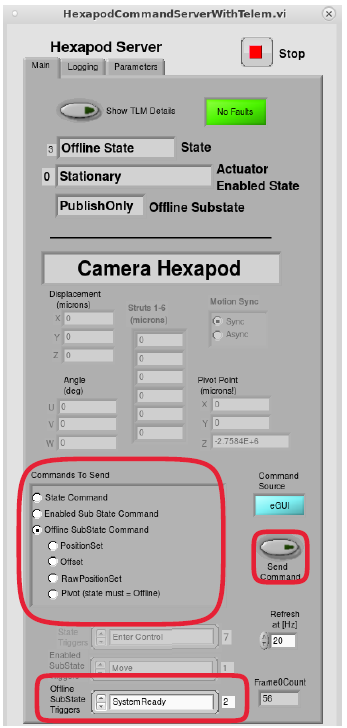
\includegraphics[width=1.79167in]{jira_imgs/1024.png}

\medskip }
\end{minipage}
\\ \cdashline{2-2}


 & Expected Result \\
 & \begin{minipage}[t]{15cm}{\footnotesize
 The system transitions from the OfflineState/PublishOnly substate to the
OfflineState/AvailableState substate.\\[2\baselineskip]

\medskip }
\end{minipage} \\ \cdashline{2-2}

 & Actual Result \\
 & \begin{minipage}[t]{15cm}{\footnotesize

\medskip }
\end{minipage} \\ \cdashline{2-2}

 & Status: \textbf{ Not Executed } \\ \hline

4 & Description \\
 & \begin{minipage}[t]{15cm}
{\footnotesize
 \textbf{SWITCHING TO DDS MODE}\\
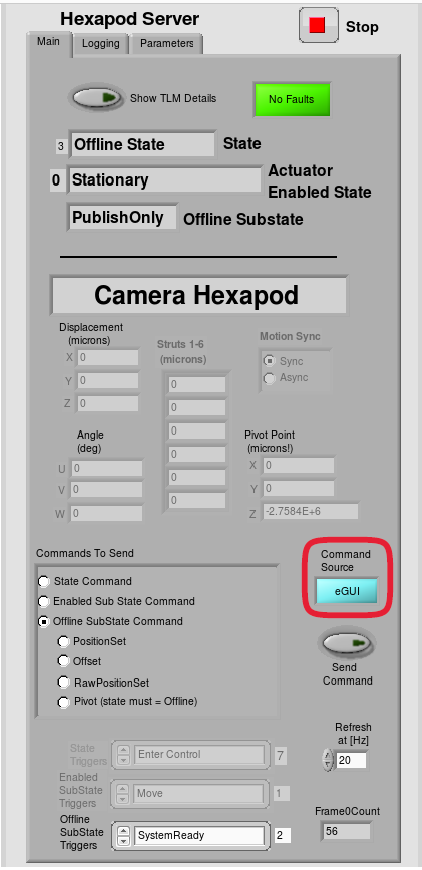
\includegraphics[width=1.68750in]{jira_imgs/1025.png}If the Command
Source does not show DDS, go to the Parameters tab, select DDS under the
Command Source and click the Set Cmd Source button.\\
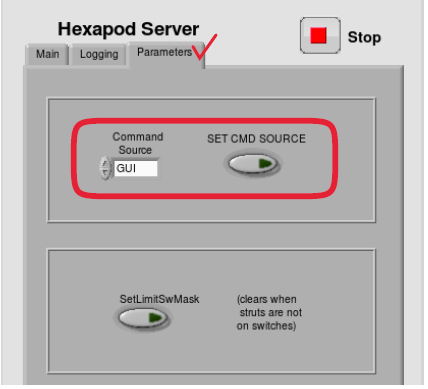
\includegraphics[width=2.34375in]{jira_imgs/1026.png}\textbf{Note:~If
the GUI is used after being set to DDS mode, the system will switch back
the Command Source to GUI and ignore any DDS commands. The Command
Source must show DDS in order to receive DDS commands.}

\medskip }
\end{minipage}
\\ \cdashline{2-2}


 & Expected Result \\
 & \begin{minipage}[t]{15cm}{\footnotesize
 The system is capable of receiving/responding to DDS commands.

\medskip }
\end{minipage} \\ \cdashline{2-2}

 & Actual Result \\
 & \begin{minipage}[t]{15cm}{\footnotesize

\medskip }
\end{minipage} \\ \cdashline{2-2}

 & Status: \textbf{ Not Executed } \\ \hline

5 & Description \\
 & \begin{minipage}[t]{15cm}
{\footnotesize
 \textbf{OFFLINESTATE -\textgreater{} STANDBYSTATE}\\
The system receives an enterControl State Transition command through
DDS.

\medskip }
\end{minipage}
\\ \cdashline{2-2}


 & Expected Result \\
 & \begin{minipage}[t]{15cm}{\footnotesize
 The system transitions into the StandbyState and is capable of
receiving/responding to DDS commands.

\medskip }
\end{minipage} \\ \cdashline{2-2}

 & Actual Result \\
 & \begin{minipage}[t]{15cm}{\footnotesize

\medskip }
\end{minipage} \\ \cdashline{2-2}

 & Status: \textbf{ Not Executed } \\ \hline

6 & Description \\
 & \begin{minipage}[t]{15cm}
{\footnotesize
 \textbf{STANDBYSTATE -\textgreater{} DISABLEDSTATE}\\
From the StandbyState, send a start command through the DDS.

\medskip }
\end{minipage}
\\ \cdashline{2-2}


 & Expected Result \\
 & \begin{minipage}[t]{15cm}{\footnotesize
 The system transitions into DisabledState after receiving/responding to
DDS command and the wrapper in the PXI real time controller looks for
the configuration file.\\[2\baselineskip]If the configuration file is
invalid or out of range, the system will transition into a Fault State

\medskip }
\end{minipage} \\ \cdashline{2-2}

 & Actual Result \\
 & \begin{minipage}[t]{15cm}{\footnotesize

\medskip }
\end{minipage} \\ \cdashline{2-2}

 & Status: \textbf{ Not Executed } \\ \hline

7 & Description \\
 & \begin{minipage}[t]{15cm}
{\footnotesize
 \textbf{DISABLEDSTATE -\textgreater{} ENABLEDSTATE}\\
From the DisabledState, send an enable state command through the DDS.\\
\textbf{}

\medskip }
\end{minipage}
\\ \cdashline{2-2}


 & Expected Result \\
 & \begin{minipage}[t]{15cm}{\footnotesize
 The system transitions into the EnabledState/Stationary substate, the
motor drives are enabled, motor brakes are released and the system is
capable of receiving/responding to DDS commands.\\[2\baselineskip]

\medskip }
\end{minipage} \\ \cdashline{2-2}

 & Actual Result \\
 & \begin{minipage}[t]{15cm}{\footnotesize

\medskip }
\end{minipage} \\ \cdashline{2-2}

 & Status: \textbf{ Not Executed } \\ \hline

8 & Description \\
 & \begin{minipage}[t]{15cm}
{\footnotesize
 \textbf{FAULTSTATE}\\
If a Fault occurs in any of the other states, the system will
automatically transition to the Fault State. While in the Fault state,
send a clearError command through the DDS.\\
Note: If the fault that occurs goes through the interlock system, reset
the safety relay switch and send a clearError command.

\medskip }
\end{minipage}
\\ \cdashline{2-2}


 & Expected Result \\
 & \begin{minipage}[t]{15cm}{\footnotesize
 The system transitions back to the OfflineState/PublishOnly substate and
is not capable of receiving/responding to DDS commands. (Go back to Step
3)

\medskip }
\end{minipage} \\ \cdashline{2-2}

 & Actual Result \\
 & \begin{minipage}[t]{15cm}{\footnotesize

\medskip }
\end{minipage} \\ \cdashline{2-2}

 & Status: \textbf{ Not Executed } \\ \hline

9 & Description \\
 & \begin{minipage}[t]{15cm}
{\footnotesize
 \textbf{{MOVE TEST}}\\
\textbf{Section 3.1.2 of the attached Software Acceptance Test
Procedure\\
Test Sequence \#1 - Synchronous PositionSet and Move Commands}\\
In enabled/stationary state, send a positionSet command of (0um, 0um,
200um, 0 deg, 0 deg, 0 deg, s).

\medskip }
\end{minipage}
\\ \cdashline{2-2}


 & Expected Result \\
 & \begin{minipage}[t]{15cm}{\footnotesize
 The hexapod does not move.

\medskip }
\end{minipage} \\ \cdashline{2-2}

 & Actual Result \\
 & \begin{minipage}[t]{15cm}{\footnotesize

\medskip }
\end{minipage} \\ \cdashline{2-2}

 & Status: \textbf{ Not Executed } \\ \hline

10 & Description \\
 & \begin{minipage}[t]{15cm}
{\footnotesize
 With the synchronous button enabled and in enabled/stationary state,
send a positionSet command of (2000um, -3500um, 200um, 0.01deg, -.05deg,
0.002deg).

\medskip }
\end{minipage}
\\ \cdashline{2-2}


 & Expected Result \\
 & \begin{minipage}[t]{15cm}{\footnotesize
 The hexapod does not move

\medskip }
\end{minipage} \\ \cdashline{2-2}

 & Actual Result \\
 & \begin{minipage}[t]{15cm}{\footnotesize

\medskip }
\end{minipage} \\ \cdashline{2-2}

 & Status: \textbf{ Not Executed } \\ \hline

11 & Description \\
 & \begin{minipage}[t]{15cm}
{\footnotesize
 Send a move command.

\medskip }
\end{minipage}
\\ \cdashline{2-2}


 & Expected Result \\
 & \begin{minipage}[t]{15cm}{\footnotesize
 \begin{itemize}
\tightlist
\item
  The hexapod moves to (2000um, -3500um, 200um, 0.01deg, -.05deg,
  0.002deg)
\item
  The actuators complete the move at nearly the same time.
\end{itemize}

\medskip }
\end{minipage} \\ \cdashline{2-2}

 & Actual Result \\
 & \begin{minipage}[t]{15cm}{\footnotesize

\medskip }
\end{minipage} \\ \cdashline{2-2}

 & Status: \textbf{ Not Executed } \\ \hline

12 & Description \\
 & \begin{minipage}[t]{15cm}
{\footnotesize
 Record the corresponding DDS events that were generated.

\medskip }
\end{minipage}
\\ \cdashline{2-2}


 & Expected Result \\
 & \begin{minipage}[t]{15cm}{\footnotesize
 \begin{itemize}
\tightlist
\item
  The controllerState.enabledSubstate goes to MOVING\_POINT\_TO\_POINT
  when the move begins and STATIONARY when the move ends.
\item
  An inPosition event is generated when the move is complete
\end{itemize}

\medskip }
\end{minipage} \\ \cdashline{2-2}

 & Actual Result \\
 & \begin{minipage}[t]{15cm}{\footnotesize

\medskip }
\end{minipage} \\ \cdashline{2-2}

 & Status: \textbf{ Not Executed } \\ \hline

13 & Description \\
 & \begin{minipage}[t]{15cm}
{\footnotesize
 \textbf{Section 3.1.2 of the attached Software Acceptance Test
Procedure\\
Test Sequence \#5 - Stop Commands}\\
In the enabled/stationary state, send a position set command of (0um,
0um, 5000um, 0deg, 0deg, 0deg)

\medskip }
\end{minipage}
\\ \cdashline{2-2}


 & Expected Result \\
 & \begin{minipage}[t]{15cm}{\footnotesize
 The hexapod doesn't move.

\medskip }
\end{minipage} \\ \cdashline{2-2}

 & Actual Result \\
 & \begin{minipage}[t]{15cm}{\footnotesize

\medskip }
\end{minipage} \\ \cdashline{2-2}

 & Status: \textbf{ Not Executed } \\ \hline

14 & Description \\
 & \begin{minipage}[t]{15cm}
{\footnotesize
 Send move command.

\medskip }
\end{minipage}
\\ \cdashline{2-2}


 & Expected Result \\
 & \begin{minipage}[t]{15cm}{\footnotesize
 The hexapod begins to move.

\medskip }
\end{minipage} \\ \cdashline{2-2}

 & Actual Result \\
 & \begin{minipage}[t]{15cm}{\footnotesize

\medskip }
\end{minipage} \\ \cdashline{2-2}

 & Status: \textbf{ Not Executed } \\ \hline

15 & Description \\
 & \begin{minipage}[t]{15cm}
{\footnotesize
 Before the hexapod completes its movement, send a stop command.

\medskip }
\end{minipage}
\\ \cdashline{2-2}


 & Expected Result \\
 & \begin{minipage}[t]{15cm}{\footnotesize
 \begin{itemize}
\tightlist
\item
  The hexapod stops before reaching the previously commanded position
\end{itemize}

\medskip }
\end{minipage} \\ \cdashline{2-2}

 & Actual Result \\
 & \begin{minipage}[t]{15cm}{\footnotesize

\medskip }
\end{minipage} \\ \cdashline{2-2}

 & Status: \textbf{ Not Executed } \\ \hline

16 & Description \\
 & \begin{minipage}[t]{15cm}
{\footnotesize
 Record the corresponding DDS events that were generated.

\medskip }
\end{minipage}
\\ \cdashline{2-2}


 & Expected Result \\
 & \begin{minipage}[t]{15cm}{\footnotesize
 \begin{itemize}
\tightlist
\item
  The controllerState.enabledSubstate goes to CONTROLLED\_STOPPING when
  the stop is requested, then STATIONARY when the hexapod has halted.
\item
  No inPosition event is generated.
\end{itemize}

\medskip }
\end{minipage} \\ \cdashline{2-2}

 & Actual Result \\
 & \begin{minipage}[t]{15cm}{\footnotesize

\medskip }
\end{minipage} \\ \cdashline{2-2}

 & Status: \textbf{ Not Executed } \\ \hline

17 & Description \\
 & \begin{minipage}[t]{15cm}
{\footnotesize
 \textbf{Section 3.1.2 of the attached Software Acceptance Test
Procedure\\
Test Sequence \#9 - positionSet and moveLUT}\\
In enabled/stationary state, send a positionSet command of (0um, 0um,
200um, 0deg, 0deg, 0deg)

\medskip }
\end{minipage}
\\ \cdashline{2-2}


 & Expected Result \\
 & \begin{minipage}[t]{15cm}{\footnotesize
 The hexapod doesn't move.

\medskip }
\end{minipage} \\ \cdashline{2-2}

 & Actual Result \\
 & \begin{minipage}[t]{15cm}{\footnotesize

\medskip }
\end{minipage} \\ \cdashline{2-2}

 & Status: \textbf{ Not Executed } \\ \hline

18 & Description \\
 & \begin{minipage}[t]{15cm}
{\footnotesize
 In enabled/stationary state, send a positionSet command of (0um, 0um,
800um, 0deg, 0deg, 0deg)

\medskip }
\end{minipage}
\\ \cdashline{2-2}


 & Expected Result \\
 & \begin{minipage}[t]{15cm}{\footnotesize
 The hexapod doesn't move.

\medskip }
\end{minipage} \\ \cdashline{2-2}

 & Actual Result \\
 & \begin{minipage}[t]{15cm}{\footnotesize

\medskip }
\end{minipage} \\ \cdashline{2-2}

 & Status: \textbf{ Not Executed } \\ \hline

19 & Description \\
 & \begin{minipage}[t]{15cm}
{\footnotesize
 Send a moveLUT (180deg, 60deg, and 10deg) command

\medskip }
\end{minipage}
\\ \cdashline{2-2}


 & Expected Result \\
 & \begin{minipage}[t]{15cm}{\footnotesize
 The hexapod moves to a different position than (0um, 0um, 800um, 0deg,
0deg, 0deg) and the actuators complete the move at nearly the same time.

\medskip }
\end{minipage} \\ \cdashline{2-2}

 & Actual Result \\
 & \begin{minipage}[t]{15cm}{\footnotesize

\medskip }
\end{minipage} \\ \cdashline{2-2}

 & Status: \textbf{ Not Executed } \\ \hline

20 & Description \\
 & \begin{minipage}[t]{15cm}
{\footnotesize
 {\textbf{OFFSET TEST}}\\
\textbf{Section 3.1.2 of the attached Software Acceptance Test
Procedure\\
Test Sequence \#4 - Synchronous Offset and Move Commands}\\
In enabled/stationary state, send a positionSet command of (500um,
800um, 200um, 0deg, 0deg, 0deg)

\medskip }
\end{minipage}
\\ \cdashline{2-2}

 & Test Data \\
 & \begin{minipage}[t]{15cm}{\footnotesize
 

\medskip }
\end{minipage} \\ \cdashline{2-2}

 & Expected Result \\
 & \begin{minipage}[t]{15cm}{\footnotesize
 The hexapod doesn't move.

\medskip }
\end{minipage} \\ \cdashline{2-2}

 & Actual Result \\
 & \begin{minipage}[t]{15cm}{\footnotesize

\medskip }
\end{minipage} \\ \cdashline{2-2}

 & Status: \textbf{ Not Executed } \\ \hline

21 & Description \\
 & \begin{minipage}[t]{15cm}
{\footnotesize
 In enabled/stationary state, send an offset command of (0um, 0um,
2000um, 0deg, 0deg, 0deg).

\medskip }
\end{minipage}
\\ \cdashline{2-2}


 & Expected Result \\
 & \begin{minipage}[t]{15cm}{\footnotesize
 The hexapod doesn't move.

\medskip }
\end{minipage} \\ \cdashline{2-2}

 & Actual Result \\
 & \begin{minipage}[t]{15cm}{\footnotesize

\medskip }
\end{minipage} \\ \cdashline{2-2}

 & Status: \textbf{ Not Executed } \\ \hline

22 & Description \\
 & \begin{minipage}[t]{15cm}
{\footnotesize
 Send a move command.~

\medskip }
\end{minipage}
\\ \cdashline{2-2}


 & Expected Result \\
 & \begin{minipage}[t]{15cm}{\footnotesize
 \begin{itemize}
\tightlist
\item
  The hexapod moves only 2000um in Z from the previous position
\item
  The actuators complete the move at nearly the same time.
\end{itemize}

\medskip }
\end{minipage} \\ \cdashline{2-2}

 & Actual Result \\
 & \begin{minipage}[t]{15cm}{\footnotesize

\medskip }
\end{minipage} \\ \cdashline{2-2}

 & Status: \textbf{ Not Executed } \\ \hline

23 & Description \\
 & \begin{minipage}[t]{15cm}
{\footnotesize
 Record the corresponding DDS events that were generated.

\medskip }
\end{minipage}
\\ \cdashline{2-2}


 & Expected Result \\
 & \begin{minipage}[t]{15cm}{\footnotesize
 \begin{itemize}
\tightlist
\item
  The controllerState.enabledSubstate goes to MOVING\_POINT\_TO\_POINT
  when the move begins and STATIONARY when the move ends
\item
  The inPosition event is True when the move finishes
\item
  The inPosition event is False when the enabledSubstate goes back to
  STATIONARY.
\end{itemize}

\medskip }
\end{minipage} \\ \cdashline{2-2}

 & Actual Result \\
 & \begin{minipage}[t]{15cm}{\footnotesize

\medskip }
\end{minipage} \\ \cdashline{2-2}

 & Status: \textbf{ Not Executed } \\ \hline

24 & Description \\
 & \begin{minipage}[t]{15cm}
{\footnotesize
 \textbf{Section 3.1.2 of the attached Software Acceptance Test
Procedure\\
Test Sequence \#2 -Pivot, PositionSet and Move Commands}\\
In enabled/stationary state, send a positionSet command of (2000um,
-3500um, 200um, 0.01deg, -0.05deg, 0.002deg)

\medskip }
\end{minipage}
\\ \cdashline{2-2}

 & Test Data \\
 & \begin{minipage}[t]{15cm}{\footnotesize
 \textbf{Deviation}: Record any offset commands necessary to test before
sending the move command.

\medskip }
\end{minipage} \\ \cdashline{2-2}

 & Expected Result \\
 & \begin{minipage}[t]{15cm}{\footnotesize
 The hexapod doesn't move.

\medskip }
\end{minipage} \\ \cdashline{2-2}

 & Actual Result \\
 & \begin{minipage}[t]{15cm}{\footnotesize

\medskip }
\end{minipage} \\ \cdashline{2-2}

 & Status: \textbf{ Not Executed } \\ \hline

25 & Description \\
 & \begin{minipage}[t]{15cm}
{\footnotesize
 In the enabled/stationary state, send a pivot command of (0,0,0).

\medskip }
\end{minipage}
\\ \cdashline{2-2}


 & Expected Result \\
 & \begin{minipage}[t]{15cm}{\footnotesize
 The actuator positions do not change but the hexapod position changes.

\medskip }
\end{minipage} \\ \cdashline{2-2}

 & Actual Result \\
 & \begin{minipage}[t]{15cm}{\footnotesize

\medskip }
\end{minipage} \\ \cdashline{2-2}

 & Status: \textbf{ Not Executed } \\ \hline

26 & Description \\
 & \begin{minipage}[t]{15cm}
{\footnotesize
 In the enabled/stationary state, send a positionSet command of (2000um,
-3500um, 200um, 0.01deg, -0.05deg, 0.002deg)

\medskip }
\end{minipage}
\\ \cdashline{2-2}

 & Test Data \\
 & \begin{minipage}[t]{15cm}{\footnotesize
 \textbf{Deviation}: Record any offset commands necessary to test before
sending the move command.

\medskip }
\end{minipage} \\ \cdashline{2-2}

 & Expected Result \\
 & \begin{minipage}[t]{15cm}{\footnotesize
 The hexapod doesn't move.

\medskip }
\end{minipage} \\ \cdashline{2-2}

 & Actual Result \\
 & \begin{minipage}[t]{15cm}{\footnotesize

\medskip }
\end{minipage} \\ \cdashline{2-2}

 & Status: \textbf{ Not Executed } \\ \hline

27 & Description \\
 & \begin{minipage}[t]{15cm}
{\footnotesize
 Send a move command.

\medskip }
\end{minipage}
\\ \cdashline{2-2}


 & Expected Result \\
 & \begin{minipage}[t]{15cm}{\footnotesize
 Confirm the hexapod moves to the commanded position and the actuators
change position to account for the new pivot point.

\medskip }
\end{minipage} \\ \cdashline{2-2}

 & Actual Result \\
 & \begin{minipage}[t]{15cm}{\footnotesize

\medskip }
\end{minipage} \\ \cdashline{2-2}

 & Status: \textbf{ Not Executed } \\ \hline

28 & Description \\
 & \begin{minipage}[t]{15cm}
{\footnotesize
 \textbf{{CONFIGURE LIMITS TEST}}\\
\textbf{Section 3.1.2 of the attached Software Acceptance Test
Procedure\\
Test Sequence \#6 - configureLimits Command}\\
In enabled/stationary state, send a configureLimits command of (12000um,
-1000um, 1000um, 0.1, -0.1, 0.05)

\medskip }
\end{minipage}
\\ \cdashline{2-2}


 & Expected Result \\
 & \begin{minipage}[t]{15cm}{\footnotesize
 The command is rejected for being outside acceptable limits.

\medskip }
\end{minipage} \\ \cdashline{2-2}

 & Actual Result \\
 & \begin{minipage}[t]{15cm}{\footnotesize

\medskip }
\end{minipage} \\ \cdashline{2-2}

 & Status: \textbf{ Not Executed } \\ \hline

29 & Description \\
 & \begin{minipage}[t]{15cm}
{\footnotesize
 In enabled/stationary state, send a configureLimits command of (1000um,
-1000um, 1000um, 0.1, -0.1, 0.05)

\medskip }
\end{minipage}
\\ \cdashline{2-2}


 & Expected Result \\
 & \begin{minipage}[t]{15cm}{\footnotesize
 The command is accepted.

\medskip }
\end{minipage} \\ \cdashline{2-2}

 & Actual Result \\
 & \begin{minipage}[t]{15cm}{\footnotesize

\medskip }
\end{minipage} \\ \cdashline{2-2}

 & Status: \textbf{ Not Executed } \\ \hline

30 & Description \\
 & \begin{minipage}[t]{15cm}
{\footnotesize
 In enabled/stationary state, send a positionSet command of (850um, 0um,
500um, 0deg, 0deg, 0deg)

\medskip }
\end{minipage}
\\ \cdashline{2-2}

 & Test Data \\
 & \begin{minipage}[t]{15cm}{\footnotesize
 \textbf{Deviation:~}This command can be any valid positionSet command
within the newly configured limits.

\medskip }
\end{minipage} \\ \cdashline{2-2}

 & Expected Result \\
 & \begin{minipage}[t]{15cm}{\footnotesize
 The command is accepted.

\medskip }
\end{minipage} \\ \cdashline{2-2}

 & Actual Result \\
 & \begin{minipage}[t]{15cm}{\footnotesize

\medskip }
\end{minipage} \\ \cdashline{2-2}

 & Status: \textbf{ Not Executed } \\ \hline

31 & Description \\
 & \begin{minipage}[t]{15cm}
{\footnotesize
 In enabled/stationary state, send a positionSet command of (1200um, 0um,
200um, 0deg, 0deg, 0deg)

\medskip }
\end{minipage}
\\ \cdashline{2-2}


 & Expected Result \\
 & \begin{minipage}[t]{15cm}{\footnotesize
 The command is rejected for being outside of range limits

\medskip }
\end{minipage} \\ \cdashline{2-2}

 & Actual Result \\
 & \begin{minipage}[t]{15cm}{\footnotesize

\medskip }
\end{minipage} \\ \cdashline{2-2}

 & Status: \textbf{ Not Executed } \\ \hline

32 & Description \\
 & \begin{minipage}[t]{15cm}
{\footnotesize
 Send a move command.

\medskip }
\end{minipage}
\\ \cdashline{2-2}


 & Expected Result \\
 & \begin{minipage}[t]{15cm}{\footnotesize
 The Hexapod doesn't move.

\medskip }
\end{minipage} \\ \cdashline{2-2}

 & Actual Result \\
 & \begin{minipage}[t]{15cm}{\footnotesize

\medskip }
\end{minipage} \\ \cdashline{2-2}

 & Status: \textbf{ Not Executed } \\ \hline

33 & Description \\
 & \begin{minipage}[t]{15cm}
{\footnotesize
 In enabled/stationary state, send a positionSet command of (990um,
990um, 200um, 0deg, 0deg, 0deg)

\medskip }
\end{minipage}
\\ \cdashline{2-2}


 & Expected Result \\
 & \begin{minipage}[t]{15cm}{\footnotesize
 The command is rejected for being outside of range limits.

\medskip }
\end{minipage} \\ \cdashline{2-2}

 & Actual Result \\
 & \begin{minipage}[t]{15cm}{\footnotesize

\medskip }
\end{minipage} \\ \cdashline{2-2}

 & Status: \textbf{ Not Executed } \\ \hline

34 & Description \\
 & \begin{minipage}[t]{15cm}
{\footnotesize
 In enabled/stationary state, send a positionSet command of (500um,
500um, 200um, 0deg, 0.1 deg, 0.01deg)

\medskip }
\end{minipage}
\\ \cdashline{2-2}


 & Expected Result \\
 & \begin{minipage}[t]{15cm}{\footnotesize
 The command is accepted.

\medskip }
\end{minipage} \\ \cdashline{2-2}

 & Actual Result \\
 & \begin{minipage}[t]{15cm}{\footnotesize

\medskip }
\end{minipage} \\ \cdashline{2-2}

 & Status: \textbf{ Not Executed } \\ \hline

35 & Description \\
 & \begin{minipage}[t]{15cm}
{\footnotesize
 Send a move command.

\medskip }
\end{minipage}
\\ \cdashline{2-2}


 & Expected Result \\
 & \begin{minipage}[t]{15cm}{\footnotesize
 The previously accepted command is executed.

\medskip }
\end{minipage} \\ \cdashline{2-2}

 & Actual Result \\
 & \begin{minipage}[t]{15cm}{\footnotesize

\medskip }
\end{minipage} \\ \cdashline{2-2}

 & Status: \textbf{ Not Executed } \\ \hline

36 & Description \\
 & \begin{minipage}[t]{15cm}
{\footnotesize
 Record the DDS events that were generated.

\medskip }
\end{minipage}
\\ \cdashline{2-2}


 & Expected Result \\
 & \begin{minipage}[t]{15cm}{\footnotesize
 The change is reflected in the settingsApplied event and the EUI.

\medskip }
\end{minipage} \\ \cdashline{2-2}

 & Actual Result \\
 & \begin{minipage}[t]{15cm}{\footnotesize

\medskip }
\end{minipage} \\ \cdashline{2-2}

 & Status: \textbf{ Not Executed } \\ \hline

37 & Description \\
 & \begin{minipage}[t]{15cm}
{\footnotesize
 {\textbf{CONFIGURE ACCELERATION TEST}}\\
\textbf{Section 3.1.2 of the attached Software Acceptance Test
Procedure\\
Test Sequence \#7 - configureAcceleration Command}\\
In enabled/stationary state, at a position of (0, 0, 0, 0, 0, 0) with
the velocity and acceleration values set to their nominal values, send a
positionSet command of (0um, 0um, 4900um, 0 deg, 0 deg, 0 deg, s).

\medskip }
\end{minipage}
\\ \cdashline{2-2}


 & Expected Result \\
 & \begin{minipage}[t]{15cm}{\footnotesize
 The hexapod doesn't move.

\medskip }
\end{minipage} \\ \cdashline{2-2}

 & Actual Result \\
 & \begin{minipage}[t]{15cm}{\footnotesize

\medskip }
\end{minipage} \\ \cdashline{2-2}

 & Status: \textbf{ Not Executed } \\ \hline

38 & Description \\
 & \begin{minipage}[t]{15cm}
{\footnotesize
 Send a move command.

\medskip }
\end{minipage}
\\ \cdashline{2-2}


 & Expected Result \\
 & \begin{minipage}[t]{15cm}{\footnotesize
 The move takes approximately 9 seconds to complete.

\medskip }
\end{minipage} \\ \cdashline{2-2}

 & Actual Result \\
 & \begin{minipage}[t]{15cm}{\footnotesize

\medskip }
\end{minipage} \\ \cdashline{2-2}

 & Status: \textbf{ Not Executed } \\ \hline

39 & Description \\
 & \begin{minipage}[t]{15cm}
{\footnotesize
 Send a configureAcceleration command of 1000.

\medskip }
\end{minipage}
\\ \cdashline{2-2}


 & Expected Result \\
 & \begin{minipage}[t]{15cm}{\footnotesize
 ~Confirm command is rejected for being outside of acceptable limits.

\medskip }
\end{minipage} \\ \cdashline{2-2}

 & Actual Result \\
 & \begin{minipage}[t]{15cm}{\footnotesize

\medskip }
\end{minipage} \\ \cdashline{2-2}

 & Status: \textbf{ Not Executed } \\ \hline

40 & Description \\
 & \begin{minipage}[t]{15cm}
{\footnotesize
 Send a configureAcceleration command of 100.

\medskip }
\end{minipage}
\\ \cdashline{2-2}


 & Expected Result \\
 & \begin{minipage}[t]{15cm}{\footnotesize
 The command is accepted.~

\medskip }
\end{minipage} \\ \cdashline{2-2}

 & Actual Result \\
 & \begin{minipage}[t]{15cm}{\footnotesize

\medskip }
\end{minipage} \\ \cdashline{2-2}

 & Status: \textbf{ Not Executed } \\ \hline

41 & Description \\
 & \begin{minipage}[t]{15cm}
{\footnotesize
 In enabled/stationary state, send a postionSet command of (0um, 0um,
0um, 0 deg, 0 deg, 0 deg, s).

\medskip }
\end{minipage}
\\ \cdashline{2-2}


 & Expected Result \\
 & \begin{minipage}[t]{15cm}{\footnotesize
 The hexapod doesn't move.

\medskip }
\end{minipage} \\ \cdashline{2-2}

 & Actual Result \\
 & \begin{minipage}[t]{15cm}{\footnotesize

\medskip }
\end{minipage} \\ \cdashline{2-2}

 & Status: \textbf{ Not Executed } \\ \hline

42 & Description \\
 & \begin{minipage}[t]{15cm}
{\footnotesize
 Send a move command.~

\medskip }
\end{minipage}
\\ \cdashline{2-2}


 & Expected Result \\
 & \begin{minipage}[t]{15cm}{\footnotesize
 It takes approximately 13 seconds to complete the commanded move with
the reduced acceleration value.

\medskip }
\end{minipage} \\ \cdashline{2-2}

 & Actual Result \\
 & \begin{minipage}[t]{15cm}{\footnotesize

\medskip }
\end{minipage} \\ \cdashline{2-2}

 & Status: \textbf{ Not Executed } \\ \hline

43 & Description \\
 & \begin{minipage}[t]{15cm}
{\footnotesize
 Send a configureAcceleration command of 500 to return the acceleration
limit to its nominal value.

\medskip }
\end{minipage}
\\ \cdashline{2-2}


 & Expected Result \\
 & \begin{minipage}[t]{15cm}{\footnotesize
 The command is accepted.

\medskip }
\end{minipage} \\ \cdashline{2-2}

 & Actual Result \\
 & \begin{minipage}[t]{15cm}{\footnotesize

\medskip }
\end{minipage} \\ \cdashline{2-2}

 & Status: \textbf{ Not Executed } \\ \hline

44 & Description \\
 & \begin{minipage}[t]{15cm}
{\footnotesize
 Record the corresponding DDS events that were generated.

\medskip }
\end{minipage}
\\ \cdashline{2-2}


 & Expected Result \\
 & \begin{minipage}[t]{15cm}{\footnotesize
 The change is reflected in the settingsApplied event and the EUI.

\medskip }
\end{minipage} \\ \cdashline{2-2}

 & Actual Result \\
 & \begin{minipage}[t]{15cm}{\footnotesize

\medskip }
\end{minipage} \\ \cdashline{2-2}

 & Status: \textbf{ Not Executed } \\ \hline

45 & Description \\
 & \begin{minipage}[t]{15cm}
{\footnotesize
 \textbf{{CONFIGURE VELOCITY TEST}}\\
\textbf{Section 3.1.2 of the attached Software Acceptance Test
Procedure\\
Test Sequence \#8 - configureVelocity Command}\\
In enabled/stationary state, at a position of (0, 0, 0, 0, 0, 0), send a
configureVelocity command of (10000, .01, 100, .01).

\medskip }
\end{minipage}
\\ \cdashline{2-2}


 & Expected Result \\
 & \begin{minipage}[t]{15cm}{\footnotesize
 This command is rejected for being outside of acceptable limits.

\medskip }
\end{minipage} \\ \cdashline{2-2}

 & Actual Result \\
 & \begin{minipage}[t]{15cm}{\footnotesize

\medskip }
\end{minipage} \\ \cdashline{2-2}

 & Status: \textbf{ Not Executed } \\ \hline

46 & Description \\
 & \begin{minipage}[t]{15cm}
{\footnotesize
 In enabled/stationary state, send a configureVelocity command of (100,
.01, 200, .01).~

\medskip }
\end{minipage}
\\ \cdashline{2-2}


 & Expected Result \\
 & \begin{minipage}[t]{15cm}{\footnotesize
 This command is accepted.

\medskip }
\end{minipage} \\ \cdashline{2-2}

 & Actual Result \\
 & \begin{minipage}[t]{15cm}{\footnotesize

\medskip }
\end{minipage} \\ \cdashline{2-2}

 & Status: \textbf{ Not Executed } \\ \hline

47 & Description \\
 & \begin{minipage}[t]{15cm}
{\footnotesize
 In enabled/stationary state, send a positionSet command of (0, 0um,
2000um, 0 deg, 0 deg, 0 deg, s).

\medskip }
\end{minipage}
\\ \cdashline{2-2}


 & Expected Result \\
 & \begin{minipage}[t]{15cm}{\footnotesize
 The command is accepted

\medskip }
\end{minipage} \\ \cdashline{2-2}

 & Actual Result \\
 & \begin{minipage}[t]{15cm}{\footnotesize

\medskip }
\end{minipage} \\ \cdashline{2-2}

 & Status: \textbf{ Not Executed } \\ \hline

48 & Description \\
 & \begin{minipage}[t]{15cm}
{\footnotesize
 Send a move command.~

\medskip }
\end{minipage}
\\ \cdashline{2-2}


 & Expected Result \\
 & \begin{minipage}[t]{15cm}{\footnotesize
 It takes approximately 20 seconds to complete the commanded move.

\medskip }
\end{minipage} \\ \cdashline{2-2}

 & Actual Result \\
 & \begin{minipage}[t]{15cm}{\footnotesize

\medskip }
\end{minipage} \\ \cdashline{2-2}

 & Status: \textbf{ Not Executed } \\ \hline

49 & Description \\
 & \begin{minipage}[t]{15cm}
{\footnotesize
 In enabled/stationary state, send a configureVelocity command of (100,
.01, 100, .01).~

\medskip }
\end{minipage}
\\ \cdashline{2-2}


 & Expected Result \\
 & \begin{minipage}[t]{15cm}{\footnotesize
 This command is accepted.

\medskip }
\end{minipage} \\ \cdashline{2-2}

 & Actual Result \\
 & \begin{minipage}[t]{15cm}{\footnotesize

\medskip }
\end{minipage} \\ \cdashline{2-2}

 & Status: \textbf{ Not Executed } \\ \hline

50 & Description \\
 & \begin{minipage}[t]{15cm}
{\footnotesize
 In enabled/stationary state, send an offset command of (0, 0um, 2000um,
0 deg, 0 deg, 0 deg).

\medskip }
\end{minipage}
\\ \cdashline{2-2}


 & Expected Result \\
 & \begin{minipage}[t]{15cm}{\footnotesize
 This command is accepted

\medskip }
\end{minipage} \\ \cdashline{2-2}

 & Actual Result \\
 & \begin{minipage}[t]{15cm}{\footnotesize

\medskip }
\end{minipage} \\ \cdashline{2-2}

 & Status: \textbf{ Not Executed } \\ \hline

51 & Description \\
 & \begin{minipage}[t]{15cm}
{\footnotesize
 Send a move command.~

\medskip }
\end{minipage}
\\ \cdashline{2-2}


 & Expected Result \\
 & \begin{minipage}[t]{15cm}{\footnotesize
 It takes approximately 40 seconds to complete the commanded move.

\medskip }
\end{minipage} \\ \cdashline{2-2}

 & Actual Result \\
 & \begin{minipage}[t]{15cm}{\footnotesize

\medskip }
\end{minipage} \\ \cdashline{2-2}

 & Status: \textbf{ Not Executed } \\ \hline

52 & Description \\
 & \begin{minipage}[t]{15cm}
{\footnotesize
 Record the corresponding DDS events that were generated:

\medskip }
\end{minipage}
\\ \cdashline{2-2}


 & Expected Result \\
 & \begin{minipage}[t]{15cm}{\footnotesize
 The change is reflected in the settingsApplied event and the EUI.

\medskip }
\end{minipage} \\ \cdashline{2-2}

 & Actual Result \\
 & \begin{minipage}[t]{15cm}{\footnotesize

\medskip }
\end{minipage} \\ \cdashline{2-2}

 & Status: \textbf{ Not Executed } \\ \hline

53 & Description \\
 & \begin{minipage}[t]{15cm}
{\footnotesize
 \textbf{Section 3.3.2 of the attached Software Acceptance Test Procedure
Hexapod Action on State Commands}\\
In the Offline/PublishOnly state, send all commands

\medskip }
\end{minipage}
\\ \cdashline{2-2}


 & Expected Result \\
 & \begin{minipage}[t]{15cm}{\footnotesize
 There is no change and command is rejected.

\medskip }
\end{minipage} \\ \cdashline{2-2}

 & Actual Result \\
 & \begin{minipage}[t]{15cm}{\footnotesize

\medskip }
\end{minipage} \\ \cdashline{2-2}

 & Status: \textbf{ Not Executed } \\ \hline

54 & Description \\
 & \begin{minipage}[t]{15cm}
{\footnotesize
 In the Offline/Available state, send an enterControl command

\medskip }
\end{minipage}
\\ \cdashline{2-2}


 & Expected Result \\
 & \begin{minipage}[t]{15cm}{\footnotesize
 The system enters the Standby state.

\medskip }
\end{minipage} \\ \cdashline{2-2}

 & Actual Result \\
 & \begin{minipage}[t]{15cm}{\footnotesize

\medskip }
\end{minipage} \\ \cdashline{2-2}

 & Status: \textbf{ Not Executed } \\ \hline

55 & Description \\
 & \begin{minipage}[t]{15cm}
{\footnotesize
 In the Standby state, send any command except start or exitControl

\medskip }
\end{minipage}
\\ \cdashline{2-2}


 & Expected Result \\
 & \begin{minipage}[t]{15cm}{\footnotesize
 There is no change and command is rejected.

\medskip }
\end{minipage} \\ \cdashline{2-2}

 & Actual Result \\
 & \begin{minipage}[t]{15cm}{\footnotesize

\medskip }
\end{minipage} \\ \cdashline{2-2}

 & Status: \textbf{ Not Executed } \\ \hline

56 & Description \\
 & \begin{minipage}[t]{15cm}
{\footnotesize
 In the Standby state, send an exitControl command.

\medskip }
\end{minipage}
\\ \cdashline{2-2}


 & Expected Result \\
 & \begin{minipage}[t]{15cm}{\footnotesize
 The system transitions into the Offline/Available state.

\medskip }
\end{minipage} \\ \cdashline{2-2}

 & Actual Result \\
 & \begin{minipage}[t]{15cm}{\footnotesize

\medskip }
\end{minipage} \\ \cdashline{2-2}

 & Status: \textbf{ Not Executed } \\ \hline

57 & Description \\
 & \begin{minipage}[t]{15cm}
{\footnotesize
 In the Standby state, send a start command.

\medskip }
\end{minipage}
\\ \cdashline{2-2}


 & Expected Result \\
 & \begin{minipage}[t]{15cm}{\footnotesize
 The system transitions into the Disabled state.

\medskip }
\end{minipage} \\ \cdashline{2-2}

 & Actual Result \\
 & \begin{minipage}[t]{15cm}{\footnotesize

\medskip }
\end{minipage} \\ \cdashline{2-2}

 & Status: \textbf{ Not Executed } \\ \hline

58 & Description \\
 & \begin{minipage}[t]{15cm}
{\footnotesize
 In the Disabled state, send any command except for the enabled or
standby command.

\medskip }
\end{minipage}
\\ \cdashline{2-2}


 & Expected Result \\
 & \begin{minipage}[t]{15cm}{\footnotesize
 There is no change and the command is rejected.

\medskip }
\end{minipage} \\ \cdashline{2-2}

 & Actual Result \\
 & \begin{minipage}[t]{15cm}{\footnotesize

\medskip }
\end{minipage} \\ \cdashline{2-2}

 & Status: \textbf{ Not Executed } \\ \hline

59 & Description \\
 & \begin{minipage}[t]{15cm}
{\footnotesize
 In the Disabled state, send the standby command.

\medskip }
\end{minipage}
\\ \cdashline{2-2}


 & Expected Result \\
 & \begin{minipage}[t]{15cm}{\footnotesize
 The system transitions into the Standby state.

\medskip }
\end{minipage} \\ \cdashline{2-2}

 & Actual Result \\
 & \begin{minipage}[t]{15cm}{\footnotesize

\medskip }
\end{minipage} \\ \cdashline{2-2}

 & Status: \textbf{ Not Executed } \\ \hline

60 & Description \\
 & \begin{minipage}[t]{15cm}
{\footnotesize
 In the Disabled state, send the enable command.

\medskip }
\end{minipage}
\\ \cdashline{2-2}


 & Expected Result \\
 & \begin{minipage}[t]{15cm}{\footnotesize
 The system transitions into the Enabled/Stationary state.

\medskip }
\end{minipage} \\ \cdashline{2-2}

 & Actual Result \\
 & \begin{minipage}[t]{15cm}{\footnotesize

\medskip }
\end{minipage} \\ \cdashline{2-2}

 & Status: \textbf{ Not Executed } \\ \hline

61 & Description \\
 & \begin{minipage}[t]{15cm}
{\footnotesize
 In the Enabled/Stationary state, send either the enterControl command,
exitControl command, start command, clearError command, or enable
command.

\medskip }
\end{minipage}
\\ \cdashline{2-2}


 & Expected Result \\
 & \begin{minipage}[t]{15cm}{\footnotesize
 There is no change and command is rejected.

\medskip }
\end{minipage} \\ \cdashline{2-2}

 & Actual Result \\
 & \begin{minipage}[t]{15cm}{\footnotesize

\medskip }
\end{minipage} \\ \cdashline{2-2}

 & Status: \textbf{ Not Executed } \\ \hline

62 & Description \\
 & \begin{minipage}[t]{15cm}
{\footnotesize
 In the Enabled/Stationary state, send a disable command.

\medskip }
\end{minipage}
\\ \cdashline{2-2}


 & Expected Result \\
 & \begin{minipage}[t]{15cm}{\footnotesize
 The system transitions into Disabled state.

\medskip }
\end{minipage} \\ \cdashline{2-2}

 & Actual Result \\
 & \begin{minipage}[t]{15cm}{\footnotesize

\medskip }
\end{minipage} \\ \cdashline{2-2}

 & Status: \textbf{ Not Executed } \\ \hline

63 & Description \\
 & \begin{minipage}[t]{15cm}
{\footnotesize
 In the Fault state, send any command except the clearError command.

\medskip }
\end{minipage}
\\ \cdashline{2-2}


 & Expected Result \\
 & \begin{minipage}[t]{15cm}{\footnotesize
 There is no change and command is rejected.

\medskip }
\end{minipage} \\ \cdashline{2-2}

 & Actual Result \\
 & \begin{minipage}[t]{15cm}{\footnotesize

\medskip }
\end{minipage} \\ \cdashline{2-2}

 & Status: \textbf{ Not Executed } \\ \hline

64 & Description \\
 & \begin{minipage}[t]{15cm}
{\footnotesize
 In the Fault state, send the clearError command.

\medskip }
\end{minipage}
\\ \cdashline{2-2}


 & Expected Result \\
 & \begin{minipage}[t]{15cm}{\footnotesize
 The system transitions into the Offline/PublishOnly state.

\medskip }
\end{minipage} \\ \cdashline{2-2}

 & Actual Result \\
 & \begin{minipage}[t]{15cm}{\footnotesize

\medskip }
\end{minipage} \\ \cdashline{2-2}

 & Status: \textbf{ Not Executed } \\ \hline

65 & Description \\
 & \begin{minipage}[t]{15cm}
{\footnotesize
 \textbf{Section 4 of the attached Software Acceptance Test Procedure}\\
In the Enabled/Stationary state, unplug a motor encoder cable for one of
the actuators.\textbf{}\\

\medskip }
\end{minipage}
\\ \cdashline{2-2}


 & Expected Result \\
 & \begin{minipage}[t]{15cm}{\footnotesize
 A Drive Fault error event is created and the system transitions to Fault
state.

\medskip }
\end{minipage} \\ \cdashline{2-2}

 & Actual Result \\
 & \begin{minipage}[t]{15cm}{\footnotesize

\medskip }
\end{minipage} \\ \cdashline{2-2}

 & Status: \textbf{ Not Executed } \\ \hline

66 & Description \\
 & \begin{minipage}[t]{15cm}
{\footnotesize
 In the Enabled/Stationary state, unplug a linear encoder cable for one
of the actuators.

\medskip }
\end{minipage}
\\ \cdashline{2-2}


 & Expected Result \\
 & \begin{minipage}[t]{15cm}{\footnotesize
 A Drive Fault error event is created and the system transitions to Fault
state.

\medskip }
\end{minipage} \\ \cdashline{2-2}

 & Actual Result \\
 & \begin{minipage}[t]{15cm}{\footnotesize

\medskip }
\end{minipage} \\ \cdashline{2-2}

 & Status: \textbf{ Not Executed } \\ \hline

67 & Description \\
 & \begin{minipage}[t]{15cm}
{\footnotesize
 Unplug a motor power cable from one of the actuators and command a
PositionSet/Move.

\medskip }
\end{minipage}
\\ \cdashline{2-2}


 & Expected Result \\
 & \begin{minipage}[t]{15cm}{\footnotesize
 A Following Error event is created and the system transitions to Fault
state.

\medskip }
\end{minipage} \\ \cdashline{2-2}

 & Actual Result \\
 & \begin{minipage}[t]{15cm}{\footnotesize

\medskip }
\end{minipage} \\ \cdashline{2-2}

 & Status: \textbf{ Not Executed } \\ \hline

68 & Description \\
 & \begin{minipage}[t]{15cm}
{\footnotesize
 Activate an extension limit switch on one of the actuators by removing
the limit switch cover and manually tripping.

\medskip }
\end{minipage}
\\ \cdashline{2-2}


 & Expected Result \\
 & \begin{minipage}[t]{15cm}{\footnotesize
 An Extended Limit Switch error event is created and the system
transitions into Fault state.

\medskip }
\end{minipage} \\ \cdashline{2-2}

 & Actual Result \\
 & \begin{minipage}[t]{15cm}{\footnotesize

\medskip }
\end{minipage} \\ \cdashline{2-2}

 & Status: \textbf{ Not Executed } \\ \hline

69 & Description \\
 & \begin{minipage}[t]{15cm}
{\footnotesize
 Activate a retraction limit switch on one of the actuators by removing
the limit switch cover and manually tripping.

\medskip }
\end{minipage}
\\ \cdashline{2-2}


 & Expected Result \\
 & \begin{minipage}[t]{15cm}{\footnotesize
 A Retracted Limit Switch error event is created and the system
transitions into Fault state.

\medskip }
\end{minipage} \\ \cdashline{2-2}

 & Actual Result \\
 & \begin{minipage}[t]{15cm}{\footnotesize

\medskip }
\end{minipage} \\ \cdashline{2-2}

 & Status: \textbf{ Not Executed } \\ \hline

70 & Description \\
 & \begin{minipage}[t]{15cm}
{\footnotesize
 Unplug the Ethercat cable between the control PC and the first Copley
XE2 drive.

\medskip }
\end{minipage}
\\ \cdashline{2-2}


 & Expected Result \\
 & \begin{minipage}[t]{15cm}{\footnotesize
 An Ethercat Lost event is created and the system transitions to Fault
state.

\medskip }
\end{minipage} \\ \cdashline{2-2}

 & Actual Result \\
 & \begin{minipage}[t]{15cm}{\footnotesize

\medskip }
\end{minipage} \\ \cdashline{2-2}

 & Status: \textbf{ Not Executed } \\ \hline

\end{longtable}


\newpage
\appendix
%Make sure lsst-texmf/bin/generateAcronyms.py is in your path
\section{Acronyms used in this document}\label{sec:acronyms}
\input{acronyms.tex}

\end{document}
